% =====================================================================
%  Where Should Drug and Protein Meet?
%  A Controlled Study of Fusion Stage in Transformer DTI Models
%
%  CSCI-2565 Machine Learning, NYU, Spring 2026
%  Authors (alphabetical): Bhavesh Gupta, Lingwei Li, Manas Ghai, Tenzin Tsundue
%  Instructor: Prof. Rajesh Ranganath
%
%  Format:  24 in (W) x 36 in (H) portrait scientific poster
%  Reading: 3 columns, strict top-to-bottom per column,
%           left-to-right column ordering (ICML / NeurIPS / ICLR style).
%  Palette: Lilac (subtle) + Okabe-Ito for the four variants.
%
%  Compile:
%     pdflatex poster.tex   (run twice for QR + cross-refs)
% =====================================================================

\documentclass[20pt, a0paper, portrait, margin=0mm,
               innermargin=6mm,
               blockverticalspace=3mm,
               colspace=5mm,
               subcolspace=3mm]{tikzposter}

% --- Paper size: 24 x 36 inches --------------------------------------
\geometry{paperwidth=24in, paperheight=36in}
\setlength{\paperwidth}{24in}
\setlength{\paperheight}{36in}
\setlength{\textwidth}{\paperwidth}
\setlength{\textheight}{\paperheight}

\makeatletter
\setlength{\TP@visibletextwidth}{\paperwidth-2\TP@innermargin}
\setlength{\TP@visibletextheight}{\paperheight-2\TP@innermargin}
\makeatother

% --- Packages --------------------------------------------------------
\usepackage[utf8]{inputenc}
\usepackage[T1]{fontenc}
\usepackage{lmodern}
\usepackage{microtype}
\usepackage{amsmath, amssymb}
\usepackage{graphicx}
\usepackage{booktabs}
\usepackage{array}
\usepackage{xcolor}
\usepackage{colortbl}
\usepackage{tikz}
\usepackage{pifont}
\usepackage{enumitem}
\usepackage{ragged2e}
\usepackage{qrcode}

\usetikzlibrary{shapes.geometric, arrows.meta, positioning, calc, backgrounds}

% --- Color palette (Lilac + Okabe-Ito) -------------------------------
\definecolor{lilacDark}{HTML}{6E4F95}    % darkest, for emphasis text
\definecolor{lilacMid}{HTML}{9B7FBF}     % block-title bars (subtle)
\definecolor{lilacLight}{HTML}{C4ABE0}   % accents
\definecolor{lilacPale}{HTML}{ECE3F5}    % callout backgrounds
\definecolor{lilacWisp}{HTML}{F7F2FB}    % subtle backgrounds
\definecolor{nyuviolet}{HTML}{57068C}    % small accent only
\definecolor{V1blue}{HTML}{0072B2}
\definecolor{V2orange}{HTML}{E69F00}
\definecolor{V3green}{HTML}{009E73}
\definecolor{V4pink}{HTML}{CC79A7}
\definecolor{accentyellow}{HTML}{F0E442}
\definecolor{accentred}{HTML}{D55E00}
\definecolor{warmgray}{HTML}{4D4D4D}

% --- Theme setup -----------------------------------------------------
\tikzposterlatexaffectionproofoff
\usetheme{Default}

\colorlet{backgroundcolor}{white}
\colorlet{framecolor}{lilacMid}
\colorlet{titlebgcolor}{lilacDark}
\colorlet{titlefgcolor}{white}
\colorlet{blocktitlebgcolor}{lilacMid}
\colorlet{blocktitlefgcolor}{white}
\colorlet{blockbodybgcolor}{white}
\colorlet{blockbodyfgcolor}{black}
\colorlet{innerblocktitlebgcolor}{lilacMid}
\colorlet{innerblocktitlefgcolor}{white}
\colorlet{notebgcolor}{lilacPale}
\colorlet{notefgcolor}{black}
\colorlet{noteframecolor}{lilacMid}

\definebackgroundstyle{NYUWhite}{
  \draw[draw=none, fill=white]
        (bottomleft) rectangle (topright);
}
\usebackgroundstyle{NYUWhite}

% --- Title ------------------------------------------------------------
\usetitlestyle{Filled}
\settitle{
  \begin{minipage}[c][1.85in][c]{0.97\paperwidth}\centering
    {\color{titlefgcolor}\fontsize{60}{70}\selectfont\bfseries
      Where Should Drug and Protein Meet?}\\[6pt]
    {\color{accentyellow}\fontsize{30}{36}\selectfont\itshape
      A Controlled Study of \textbf{Fusion Stage} in Transformer DTI Models}\\[10pt]
    {\color{titlefgcolor}\fontsize{19}{23}\selectfont
      \textbf{Bhavesh Gupta} \,\textbullet\, \textbf{Lingwei Li}
      \,\textbullet\, \textbf{Manas Ghai} \,\textbullet\, \textbf{Tenzin Tsundue}
      \quad\textbar\quad
      NYU Courant Institute of Mathematical Sciences
      \quad\textbar\quad
      CSCI-2565 \emph{Machine Learning} (Spring 2026)}\\[8pt]
    {\color{titlefgcolor}\fontsize{17}{21}\selectfont
      Instructor: \textbf{Prof.\ Rajesh Ranganath}
      \quad\textbullet\quad
      TAs: Nhi Nguyen \,\textbullet\, Riya Mahesh \,\textbullet\, Siddhant Mohan}
  \end{minipage}
}

% Tighter custom block style (less padding -> more content per block)
\defineblockstyle{Tight}{
  titlewidthscale=1, bodywidthscale=1,
  titlecenter, titleoffsetx=0pt, titleoffsety=0pt,
  bodyoffsetx=0pt, bodyoffsety=0pt,
  bodyverticalshift=0mm, roundedcorners=8, linewidth=1.5pt,
  titleinnersep=4mm, bodyinnersep=4mm
}{
  \draw[color=lilacMid, fill=blockbodybgcolor, line width=1.5pt,
        rounded corners=6pt]
       (blockbody.south west) rectangle (blockbody.north east);
  \ifBlockHasTitle
    \draw[draw=none, fill=lilacMid, rounded corners=6pt]
       (blocktitle.south west) rectangle (blocktitle.north east);
    \fill[lilacMid] ($(blocktitle.south west)$)
                    rectangle ($(blocktitle.south east) + (0,6pt)$);
  \fi
}
\useblockstyle{Tight}
\useinnerblockstyle{Default}

% --- Helper macros ---------------------------------------------------
\newcommand{\cmark}{\textcolor{V3green}{\ding{51}}}
\newcommand{\xmark}{\textcolor{accentred}{\ding{55}}}
\newcommand{\partialmark}{\textcolor{V2orange}{$\sim$}}

\newcommand{\Vone}{\textcolor{V1blue}{\textbf{V1}}}
\newcommand{\Vtwo}{\textcolor{V2orange}{\textbf{V2}}}
\newcommand{\Vthree}{\textcolor{V3green}{\textbf{V3}}}
\newcommand{\Vfour}{\textcolor{V4pink}{\textbf{V4}}}

\newcommand{\bodysize}{\fontsize{14}{18}\selectfont}
\newcommand{\smallbody}{\fontsize{13}{16}\selectfont}
\newcommand{\capsize}{\fontsize{11}{14}\selectfont}
% Sub-heading inside a block (replaces individual block titles)
\newcommand{\subhead}[1]{\par\medskip%
  \noindent{\fontsize{18}{22}\selectfont\bfseries\color{lilacDark}#1}%
  \par\smallskip}
\newcommand{\subheadFirst}[1]{%
  \noindent{\fontsize{18}{22}\selectfont\bfseries\color{lilacDark}#1}%
  \par\smallskip}

\newcommand{\figcap}[1]{\par\vspace{1mm}{\capsize\itshape\color{warmgray}#1\par}}

\newcommand{\callout}[1]{%
  \par\smallskip
  \fcolorbox{lilacMid}{lilacPale}{%
    \begin{minipage}{0.96\linewidth}\vspace{1mm}#1\vspace{1mm}\end{minipage}}\par
  \smallskip}

\newcommand{\highlight}[1]{%
  \par\smallskip
  \fcolorbox{lilacMid}{accentyellow!50}{%
    \begin{minipage}{0.96\linewidth}\vspace{1mm}\centering#1\vspace{1mm}\end{minipage}}\par
  \smallskip}

% =====================================================================
\begin{document}
\maketitle[width=\paperwidth, titletoblockverticalspace=8mm]

% =====================================================================
% 3 STRICT TOP-TO-BOTTOM COLUMNS (ICML / NeurIPS reading order)
%   COL 1 = WHY    -> abstract, motivation, Q & H, background, hero, contrast
%   COL 2 = HOW    -> single Methodology mega-block (5 sub-heads)
%   COL 3 = WHAT   -> results + deep analysis, findings + conclusions,
%                     limitations + future, acks + refs + repo
% =====================================================================
\begin{columns}

% =====================================================================
%  COLUMN 1 --- WHY
% =====================================================================
\column{0.33}

\block{1.\ Abstract}{%
  \bodysize
  Predicting drug--protein binding affinity is foundational in
  computational drug discovery. Modern transformer DTI predictors
  uniformly fuse drug and protein representations \emph{late} ---
  after independent encoding --- but this design choice has rarely
  been audited. We construct a $2\times 2$ controlled experiment
  (concatenation vs cross-attention $\times$ before vs after
  encoding), train all four variants on \textbf{27{,}715} BindingDB
  Ki measurements under matched hyperparameters
  ($d{=}128$, $h{=}4$, lr$\,{=}3{\times}10^{-4}$, dropout$\,{=}0.1$,
  30 epochs), and evaluate across random, cold-drug, and cold-target
  splits with three seeds each \textbf{(36 runs total)}.
  \textbf{Each split has a different winner: \Vtwo\ (early X-attn) wins
  random and cold-target; \Vthree\ (late X-attn) wins cold-drug; the
  field-default \Vfour\ (late concat) never wins.} Linear CKA on
  attention features shows the variants cluster by \emph{fusion
  stage} (early vs late, CKA $\geq 0.95$ within), not by
  \emph{fusion mechanism} --- the $2\times 2$ collapses behaviorally
  to a $1\times 2$.
  \highlight{\fontsize{17}{21}\selectfont\bfseries\color{lilacDark}
    We're not claiming better numbers than the SOTA. We're claiming
    that the field's default architecture is wrong --- with proper
    controls to back it up.}
}

\block{2.\ Motivation \& the Gap}{%
  \bodysize
  \begin{itemize}[leftmargin=0.6cm, itemsep=2pt, topsep=1pt]
    \item DTI shrinks the funnel from \textbf{billions} of candidate
          molecules to a wet-lab shortlist. AI-in-drug-discovery
          market: \textbf{\$13--20 B by 2030}; \textbf{75+}
          AI-discovered candidates in clinical trials by end-2024
          (DSP-1181, INS018\_055).
    \item Transformer encoders dominate state-of-the-art DTI ---
          but the field has converged on a single design pattern
          (encode separately, fuse late) without rigorous
          justification. MolTrans, DeepPurpose, HyperAttentionDTI,
          PerceiverCPI, DrugBAN, FusionDTI all share this pattern.
    \item \textbf{The gap.} Architecture-comparison studies vary
          \emph{which encoder} (CNN vs Transformer vs GNN). Almost
          \emph{none} vary \emph{where} the modalities interact.
          We isolate that single axis under matched hyperparameters,
          matched data, matched optimizer.
    \item \textbf{Cost of an unaudited default.} Every downstream
          paper inherits it. A 15--17\,\% relative MSE gap on the
          deployment-realistic split compounds across the entire
          field.
  \end{itemize}
}

\block{3.\ Research Hypotheses}{%
  \bodysize
  \textit{When a transformer predicts drug--protein binding affinity,
  does the \textbf{stage} at which drug and protein representations
  interact materially affect (a) accuracy, (b) generalization to
  unseen drugs / targets, and (c) what the model learns?}\par\smallskip

  \smallbody
  \renewcommand{\arraystretch}{1.18}
  \setlength{\tabcolsep}{3pt}
  \begin{tabular}{@{}p{0.5cm} p{12.0cm} p{2.5cm}@{}}
  \toprule
  \textbf{H} & \textbf{Statement} & \textbf{Status} \\
  \midrule
  H1 & Late fusion (\Vthree, \Vfour) is the field default but is
       \textbf{not} Pareto-optimal across splits.
     & \cmark\ Confirmed \\
  H2 & Cross-attention recovers more biologically meaningful
       structure than concatenation.
     & \partialmark\ Partial \\
  H3 & Early fusion is more parameter-efficient at matched accuracy.
     & \cmark\ Confirmed \\
  H4 & All 4 variants converge to similar internal representations
       (CKA $\gtrsim$ 0.8) under matched compute.
     & \xmark\ \textbf{Refuted} \\
  \bottomrule
  \end{tabular}
}

\block{4.\ Background \& Prior Art}{%
  \bodysize
  \textbf{DTI = regression over pKi / pKd / pIC50.} Standard
  benchmarks: Davis (442 kinases $\times$ 379 drugs), KIBA
  (2{,}116 $\times$ 229), BindingDB ($\sim$2\,M measurements).
  Drugs $\to$ SMILES; proteins $\to$ amino-acid sequences (or 3D
  structure when available).\par\smallskip
  \textbf{Transformer DTI canon} (MolTrans, DeepPurpose,
  HyperAttentionDTI, PerceiverCPI, DrugBAN, TransformerCPI,
  FusionDTI) --- all converge on independent encoding then late
  fusion.\par\smallskip
  \textbf{Known reproducibility issue.} Most DTI papers headline
  \emph{random-split} numbers; cold-drug / cold-target performance
  is 10--25 CI points lower (Pahikkala 2015, Mayr 2018, Chen 2021).
  We report all three splits to surface the deployment-realistic gap.
}

\block{5.\ The 2$\times$2 Design --- Hero}{%
  \centering
  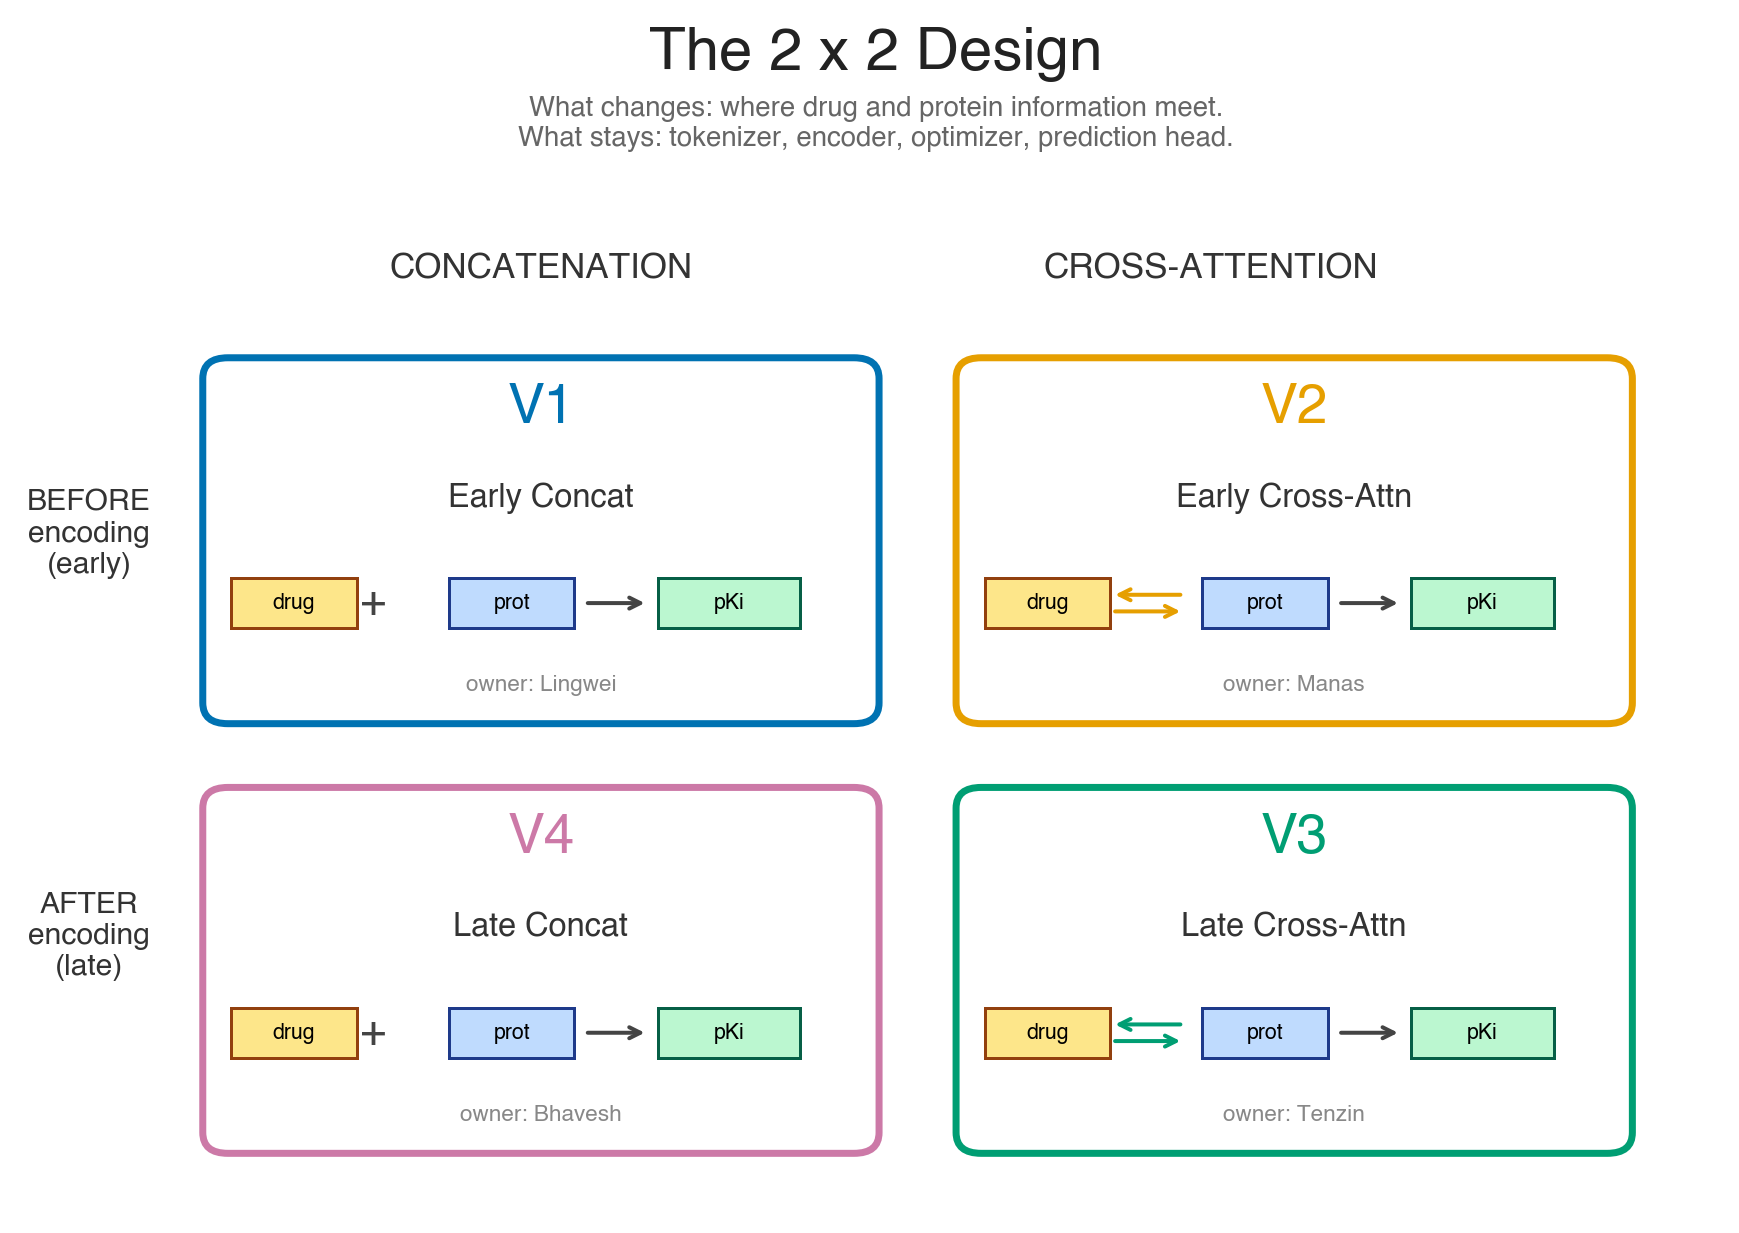
\includegraphics[width=0.99\linewidth]{poster_figures/diagram_03_matrix.png}
  \figcap{\textbf{The hero.} Hold every other component constant
  (encoder, optimizer, head, data, tokenizers); vary only
  \textbf{where} (rows: before / after encoding) and \textbf{how}
  (columns: concat / X-attn) drug + protein representations meet.}
}

\block{6.\ What We Did Differently}{%
  \centering
  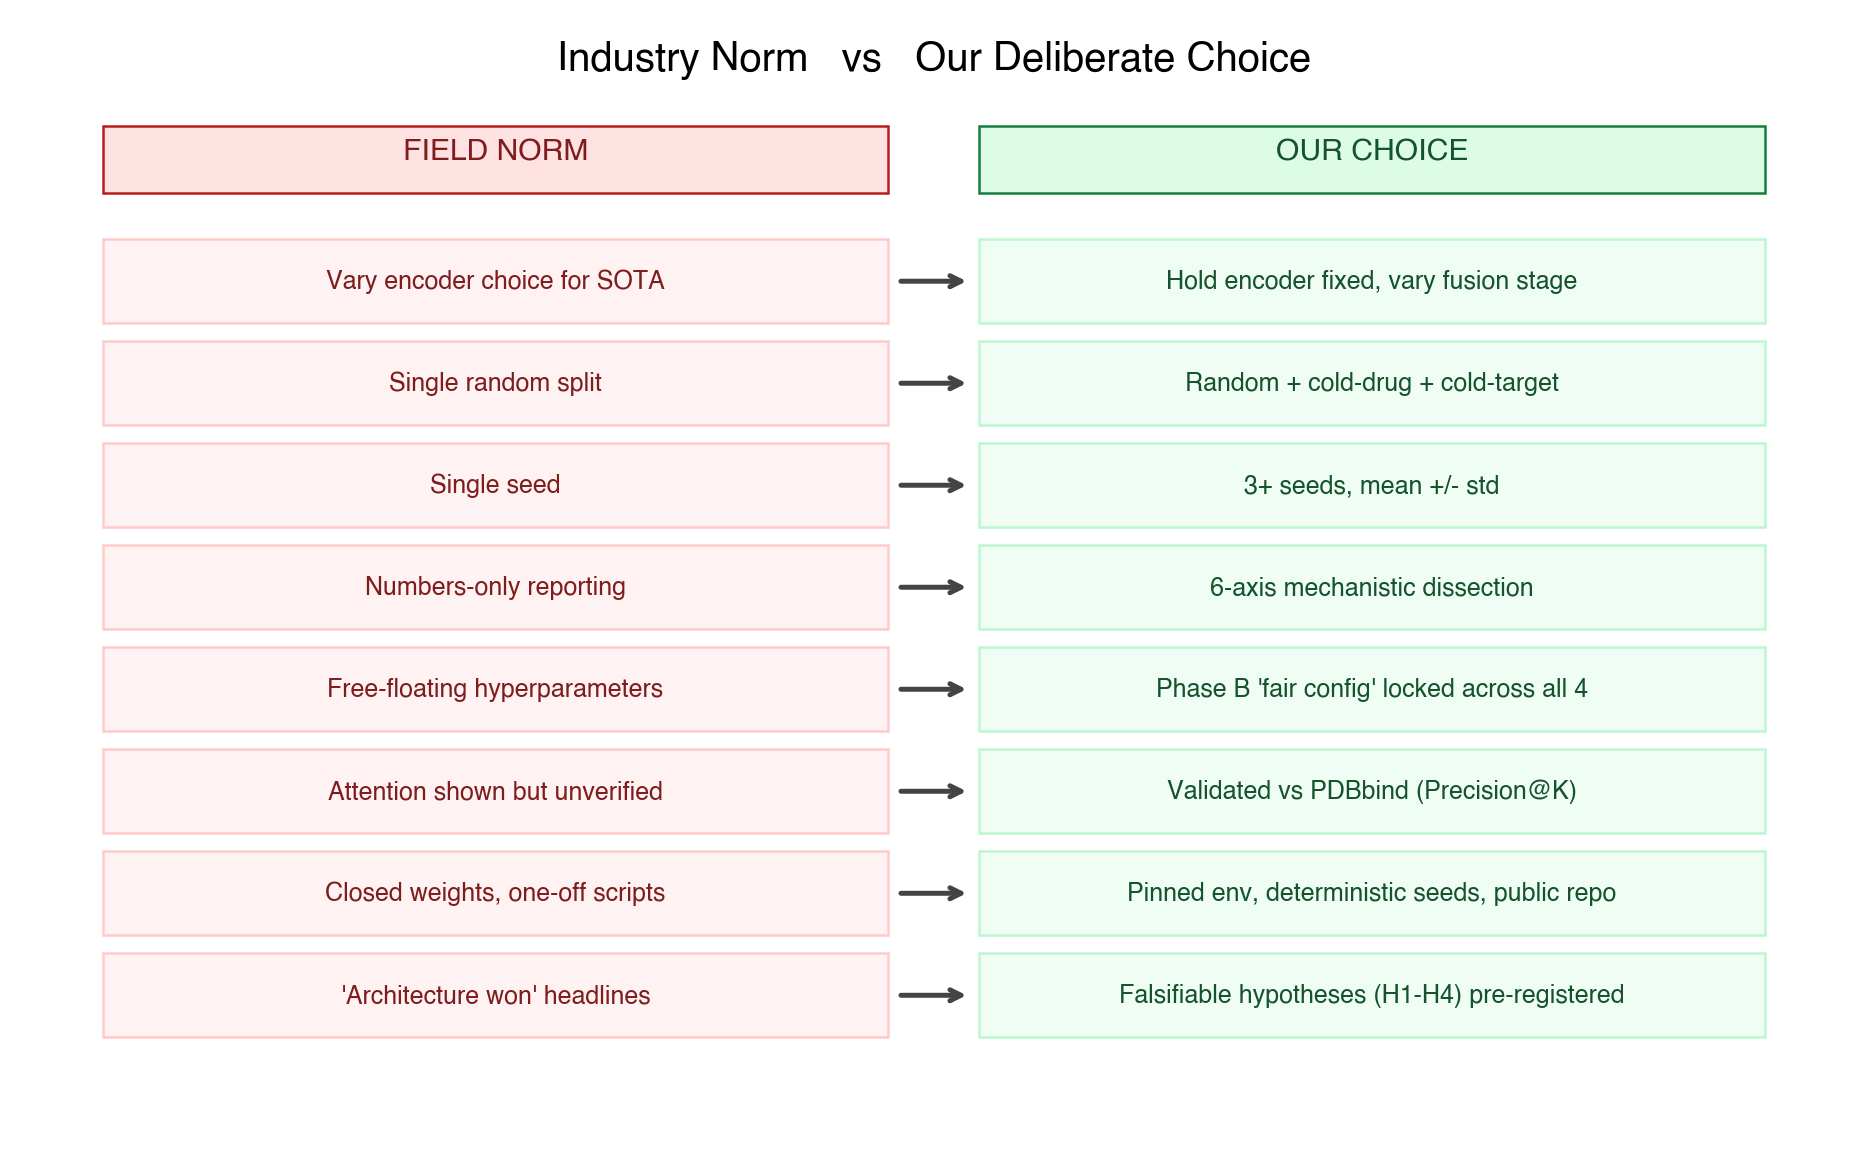
\includegraphics[width=0.99\linewidth]{poster_figures/diagram_37_norm_vs_us.png}
  \figcap{Field norm \emph{vs} our deliberate choice across 8 axes:
  hold encoder fixed, three splits not one, three seeds with mean
  $\pm$ std reporting, six-axis mechanistic dissection, fully
  reproducible repo.}
}

\block{Scan for Code}{%
  \centering
  \fcolorbox{lilacMid}{lilacWisp}{%
    \begin{minipage}{0.99\linewidth}\centering\vspace{2mm}
      \begin{minipage}[c]{0.30\linewidth}\centering
        \qrset{height=1.05in}
        \qrcode[level=H]{https://github.com/bhaveshgupta01/ComparisionPDI}
      \end{minipage}\hfill
      \begin{minipage}[c]{0.66\linewidth}\raggedright
        \fontsize{15}{19}\selectfont\bfseries\color{lilacDark}
        Code, configs, checkpoints, all 27 figures.\par
        \vspace{1.5mm}
        \fontsize{12}{15}\selectfont\ttfamily\mdseries\color{warmgray}
        github.com/bhaveshgupta01/ComparisionPDI\par
        \vspace{1.5mm}
        \fontsize{11}{14}\selectfont\rmfamily\itshape\color{warmgray}
        Scan to explore the repo.
      \end{minipage}\par\vspace{2mm}
    \end{minipage}}%
}

% =====================================================================
%  COLUMN 2 --- HOW (single big Methodology block)
% =====================================================================
\column{0.34}

\block{7.\ Methodology}{%
  % --- a) Four Variants -------------------------------------------------
  \subheadFirst{a) Four Variants, One Controlled Axis}
  \centering
  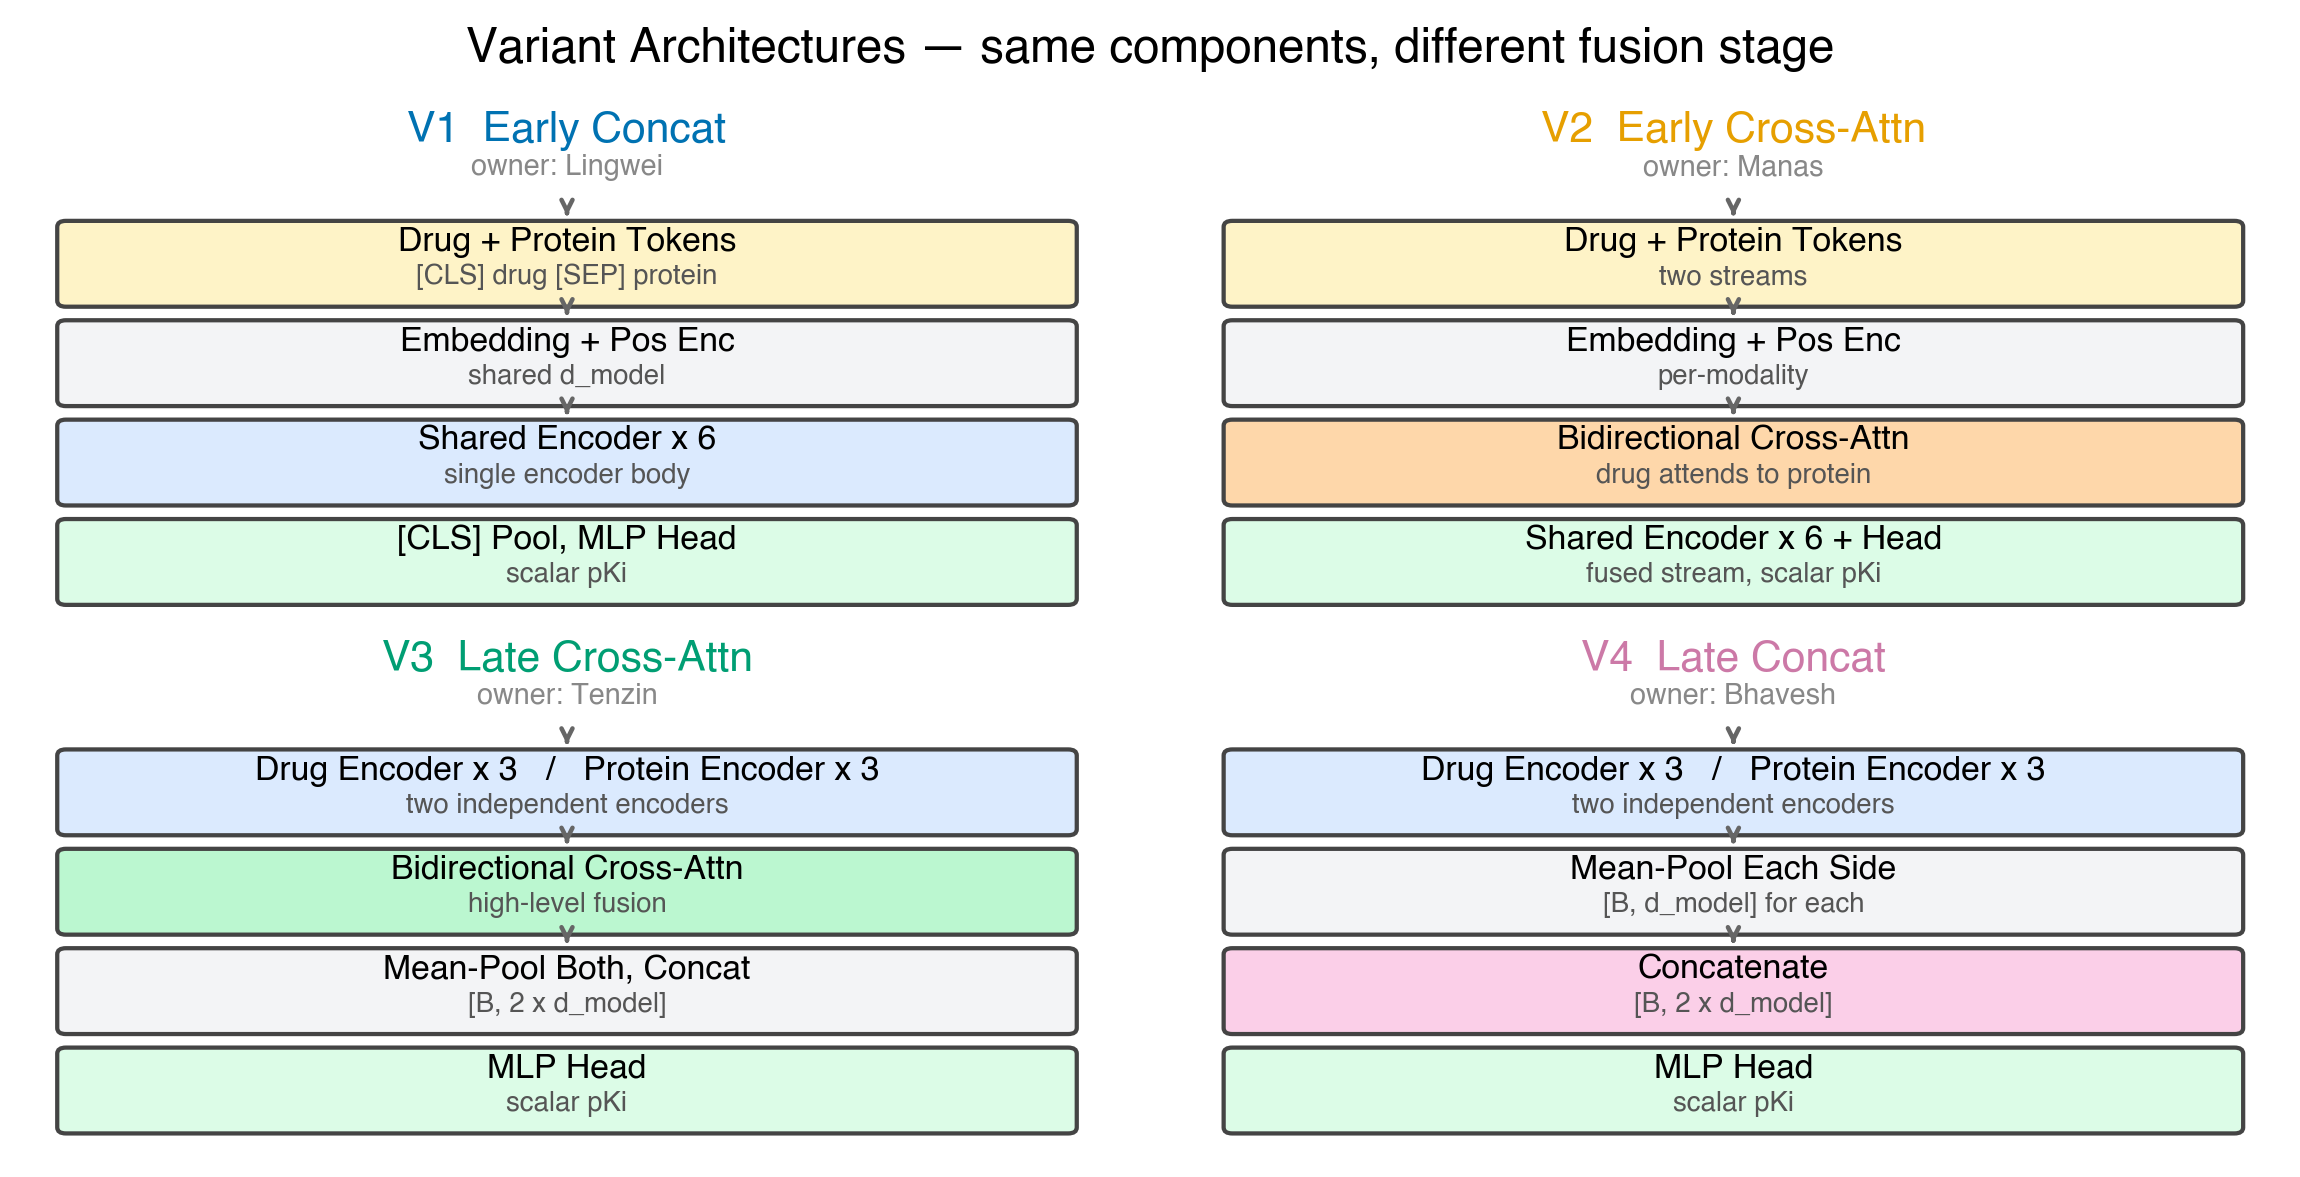
\includegraphics[width=0.99\linewidth]{poster_figures/diagram_04_architectures.png}\par\smallskip
  \smallbody\raggedright
  \begin{itemize}[leftmargin=0.6cm, itemsep=1pt, topsep=2pt]
    \item \Vone\ \textbf{Early Concat}.
      {\small\textsc{[CLS, drug, SEP, protein]}} $\to$ shared 6-layer
      pre-norm transformer encoder $\to$ CLS pool $\to$ MLP head.
      \textbf{1.27\,M params (cheapest).}
    \item \Vtwo\ \textbf{Early Cross-Attn}. Embedded drug /
      protein streams exchange info via bidirectional X-attn
      \emph{before} a 6-layer shared encoder consumes the fused
      stream. \textbf{1.40\,M.}
    \item \Vthree\ \textbf{Late Cross-Attn}. Independent
      3-layer encoders $\to$ bidirectional X-attn $\to$ mean-pool
      both $\to$ concat $\to$ MLP. \textbf{1.40\,M.}
    \item \Vfour\ \textbf{Late Concat}. Independent 3-layer
      encoders $\to$ mean-pool $\to$ concat pooled vectors $\to$ MLP.
      \textbf{1.20\,M. The field default.}
  \end{itemize}\par
  \figcap{\textbf{The control argument.} All four variants share the
  \textbf{same} encoder block, tokenizers, optimizer, head, and
  loss. Only fusion stage and mechanism change --- so any
  performance gap attributes cleanly to the fusion axis.}

  % --- b) Shared Encoder ------------------------------------------------
  \subhead{b) Shared Encoder Block (the Control)}
  \centering
  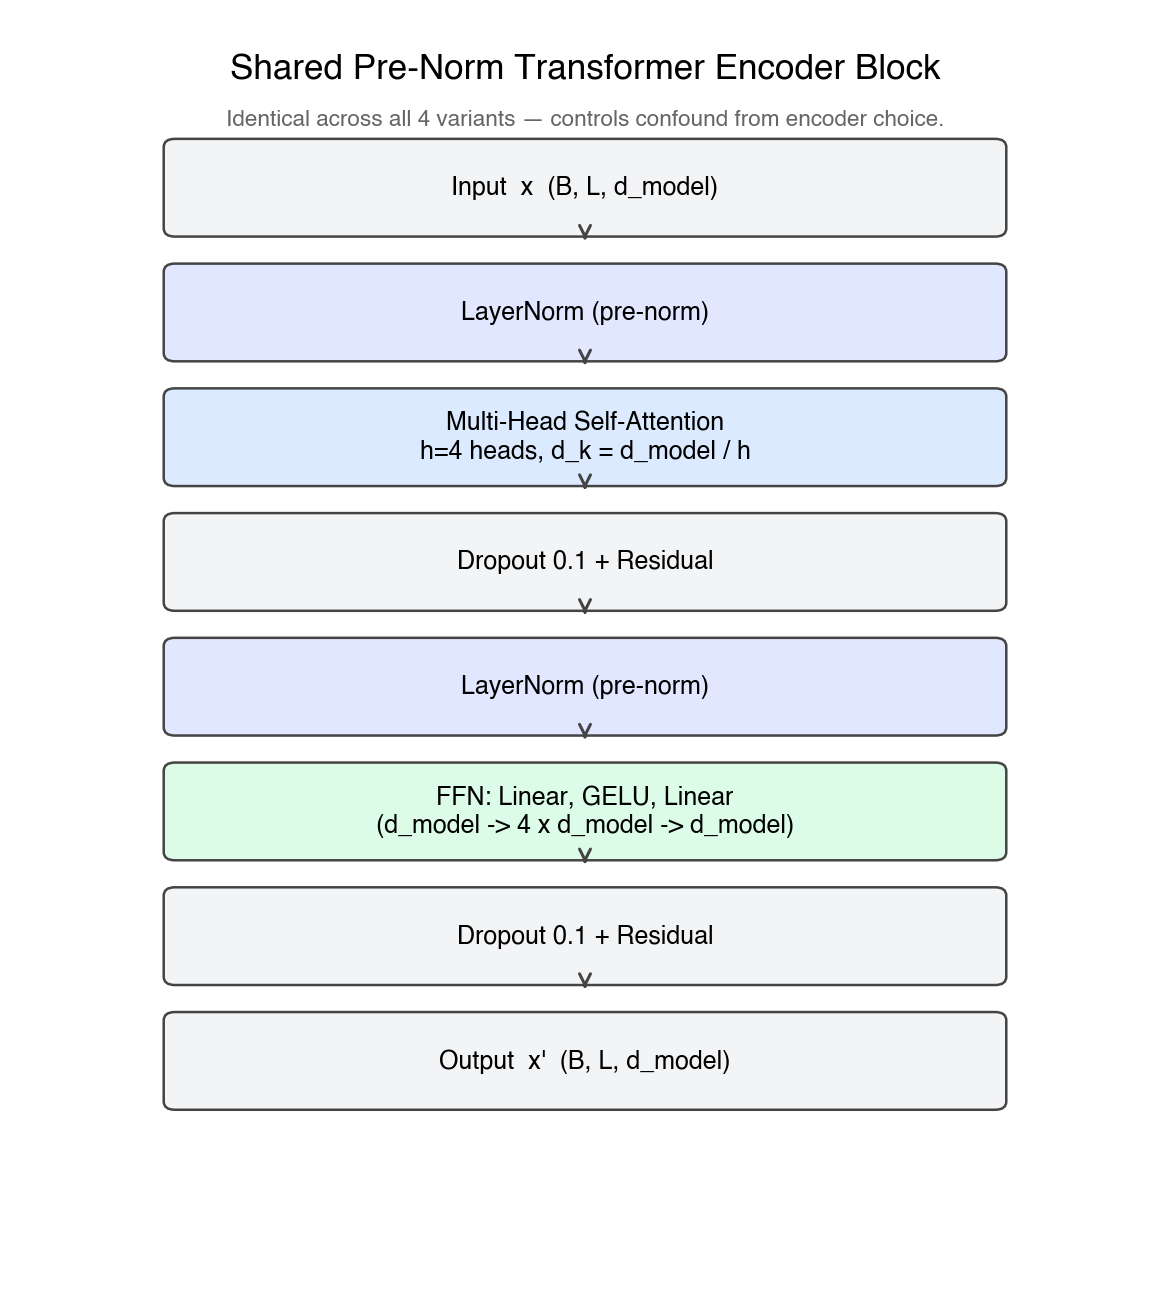
\includegraphics[width=0.55\linewidth]{poster_figures/diagram_05_encoder_block.png}\par\smallskip
  \smallbody
  \renewcommand{\arraystretch}{1.10}
  \setlength{\tabcolsep}{3pt}
  \begin{tabular}{@{}p{4.6cm} p{11.5cm}@{}}
  \toprule
  Drug tokenizer       & SMILES regex, $\sim$70 tokens \\
  Protein tokenizer    & Char-level, 25 tokens (20 AA + special) \\
  Position encoding    & Sinusoidal (Vaswani 2017) \\
  Encoder block        & Pre-norm Transformer (LN $\to$ Attn $\to$ FFN, residuals) \\
  Pooling              & Mean over non-pad tokens (or {\small\textsc{[CLS]}} for \Vone) \\
  Head                 & 2-layer MLP, GELU, dropout 0.1, scalar pKi \\
  Loss / Optim.        & MSE on pKi / AdamW + cosine + warmup \\
  \bottomrule
  \end{tabular}

  % --- c) Data ----------------------------------------------------------
  \subhead{c) Data --- BindingDB Ki (PDSP)}
  \centering
  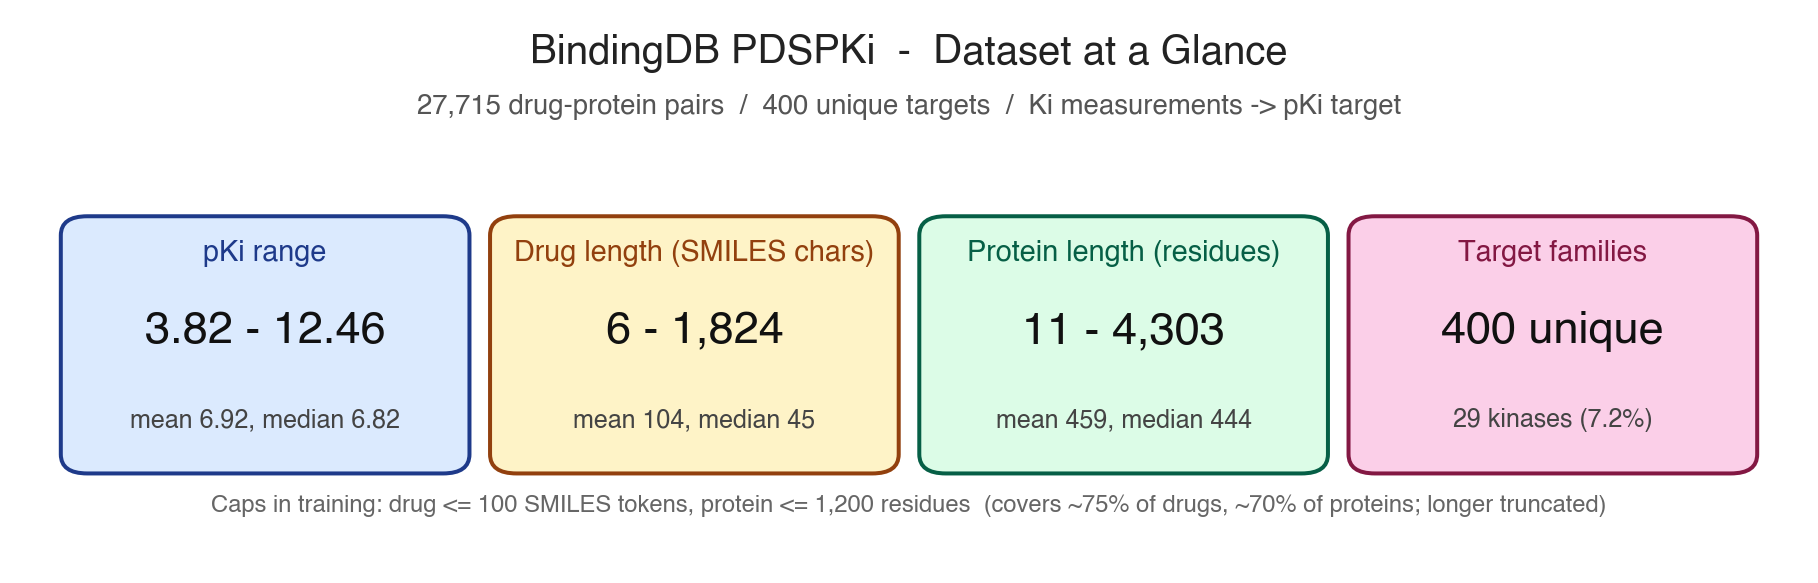
\includegraphics[width=0.85\linewidth]{poster_figures/diagram_06_dataset_summary.png}\par\smallskip
  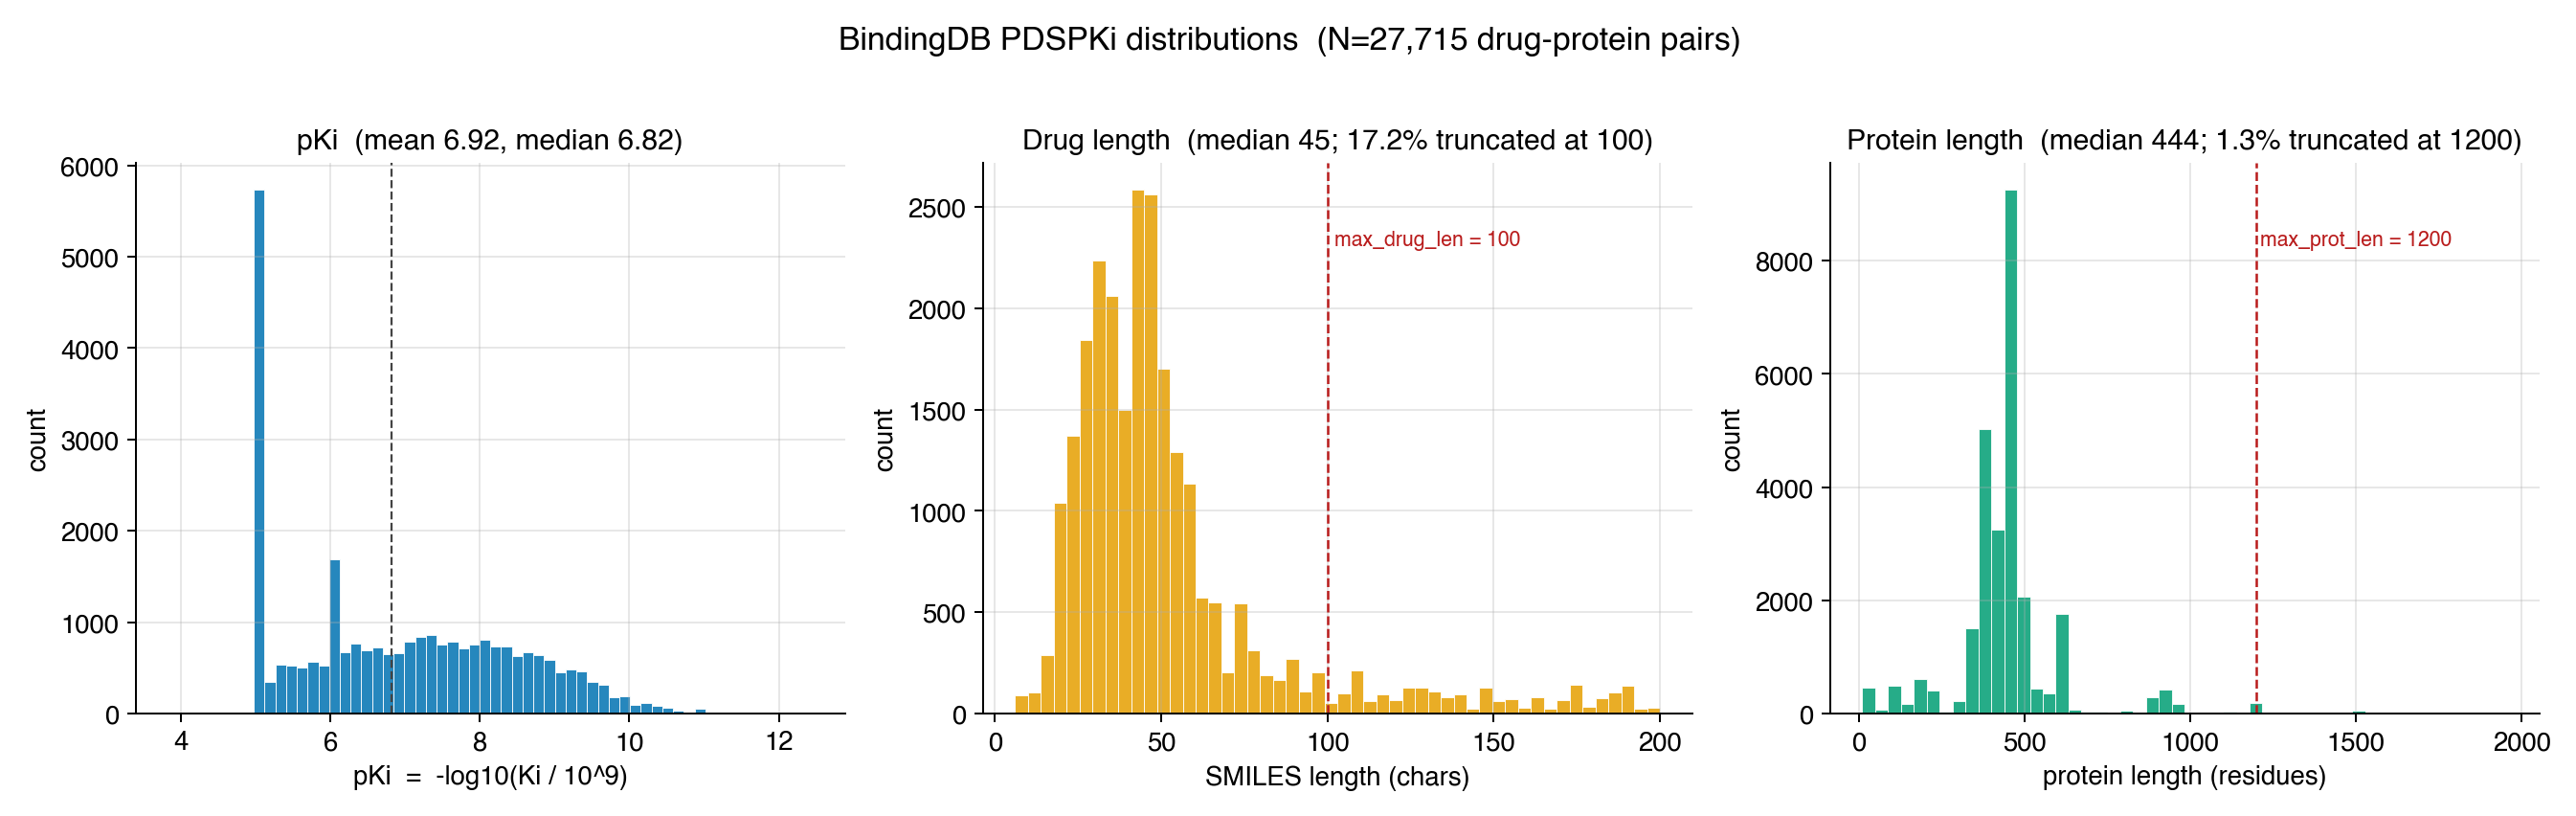
\includegraphics[width=0.85\linewidth]{poster_figures/diagram_07_length_and_pki_distribution.png}\par\smallskip
  \smallbody\raggedright
  \textbullet\ \textbf{27{,}715 pairs.} pKi $= -\log_{10}(K_i / 10^9)
  \in [3, 12]$. Caps: drug $\leq$ 100 tokens; protein $\leq$ 1200 res.
  Censored: 21\,\% at pKi $= 5.0$; 17\,\% drugs / 1\,\% proteins
  truncated.

  % --- d) Three Splits --------------------------------------------------
  \subhead{d) Three Splits --- Random + Two Cold}
  \centering
  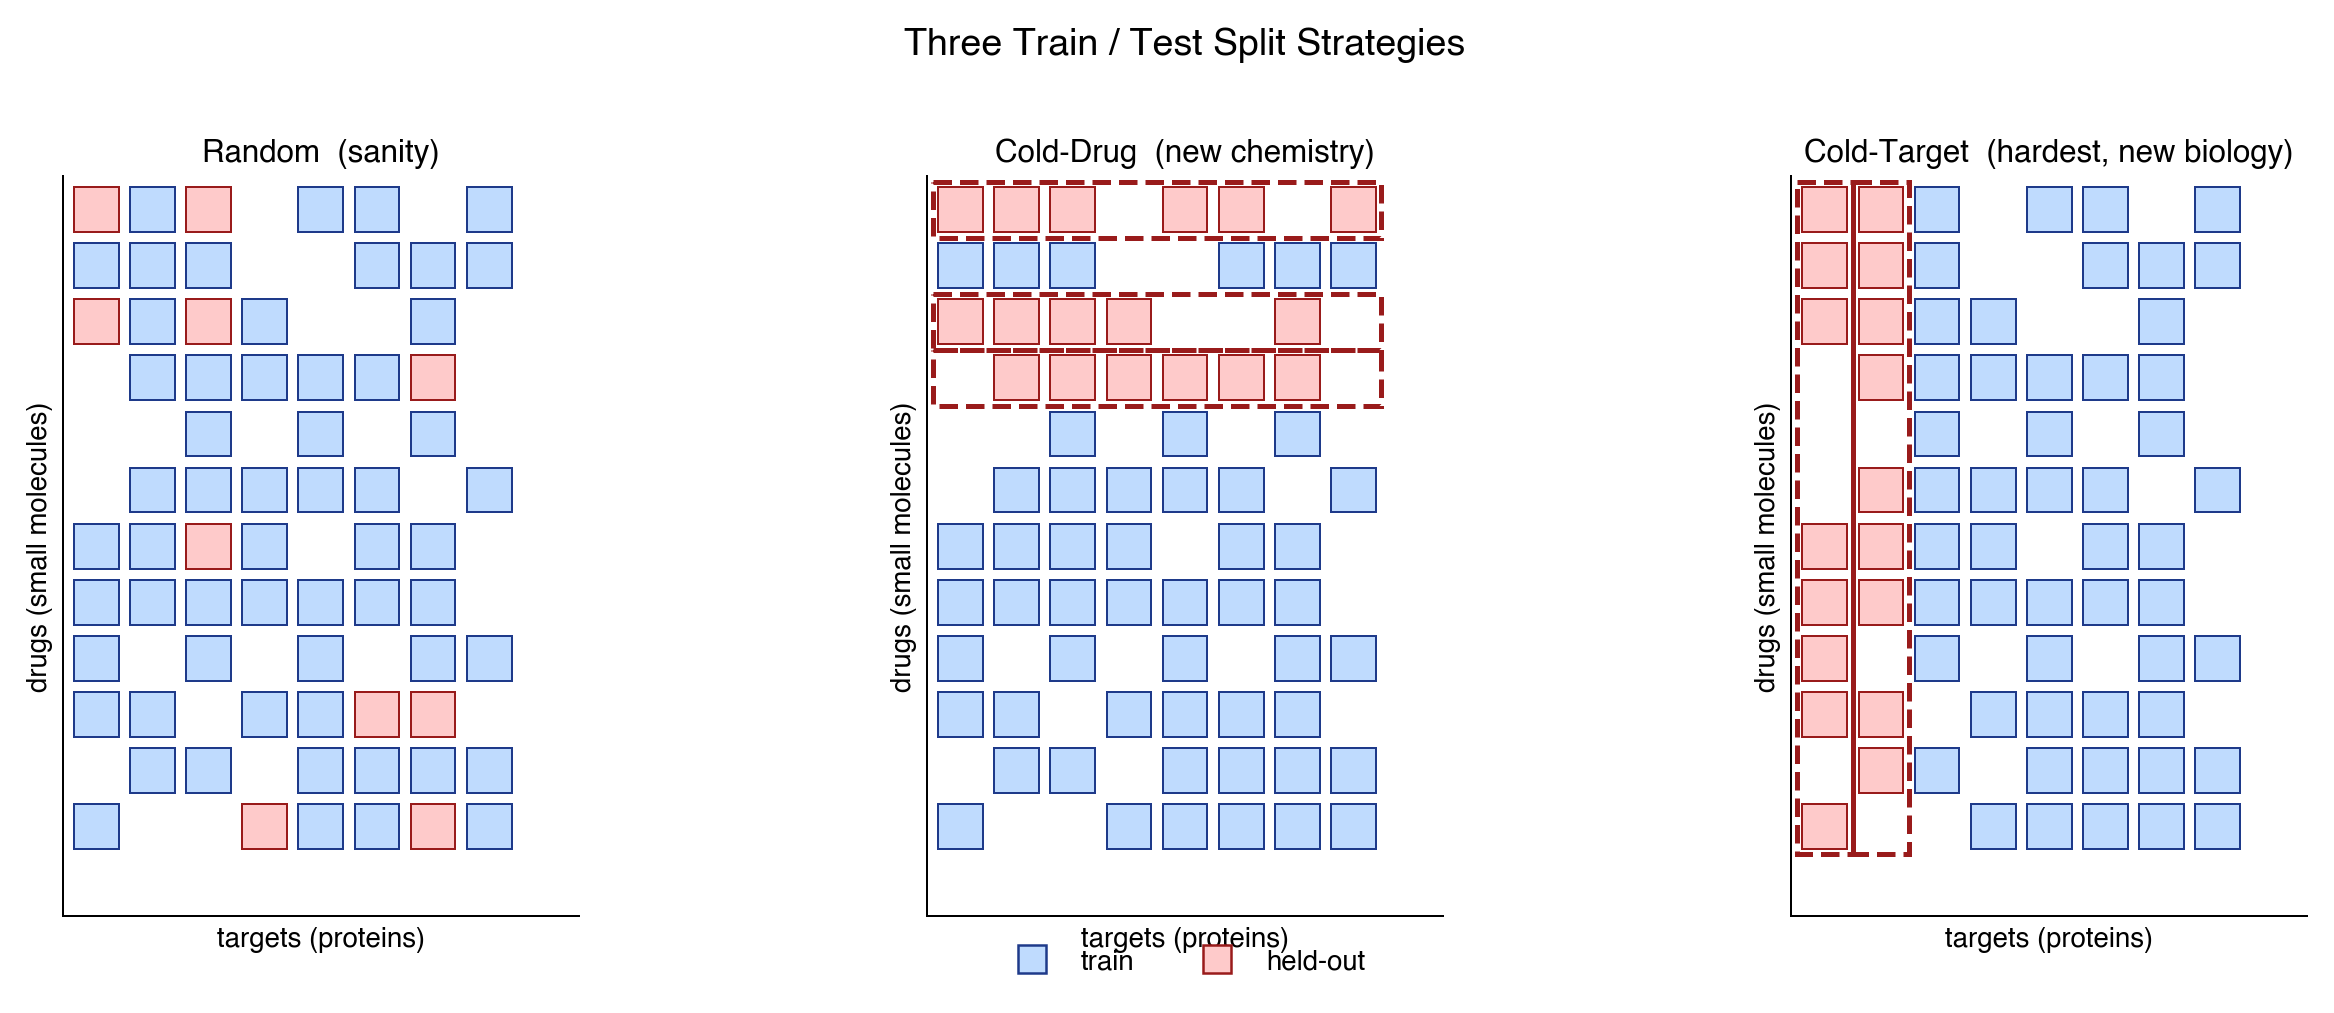
\includegraphics[width=0.92\linewidth]{poster_figures/diagram_08_split_strategy.png}
  \figcap{\textbf{Random 80/10/10} (sanity), \textbf{Cold-Drug}
  (new chemistry), \textbf{Cold-Target} (new biology, hardest).
  Cold splits are \textbf{40\,\%} harder on average --- the
  inflation that random-split-only DTI papers hide.}

  % --- e) Four-Phase Protocol ------------------------------------------
  \subhead{e) Four-Phase Protocol \& Compute}
  \centering
  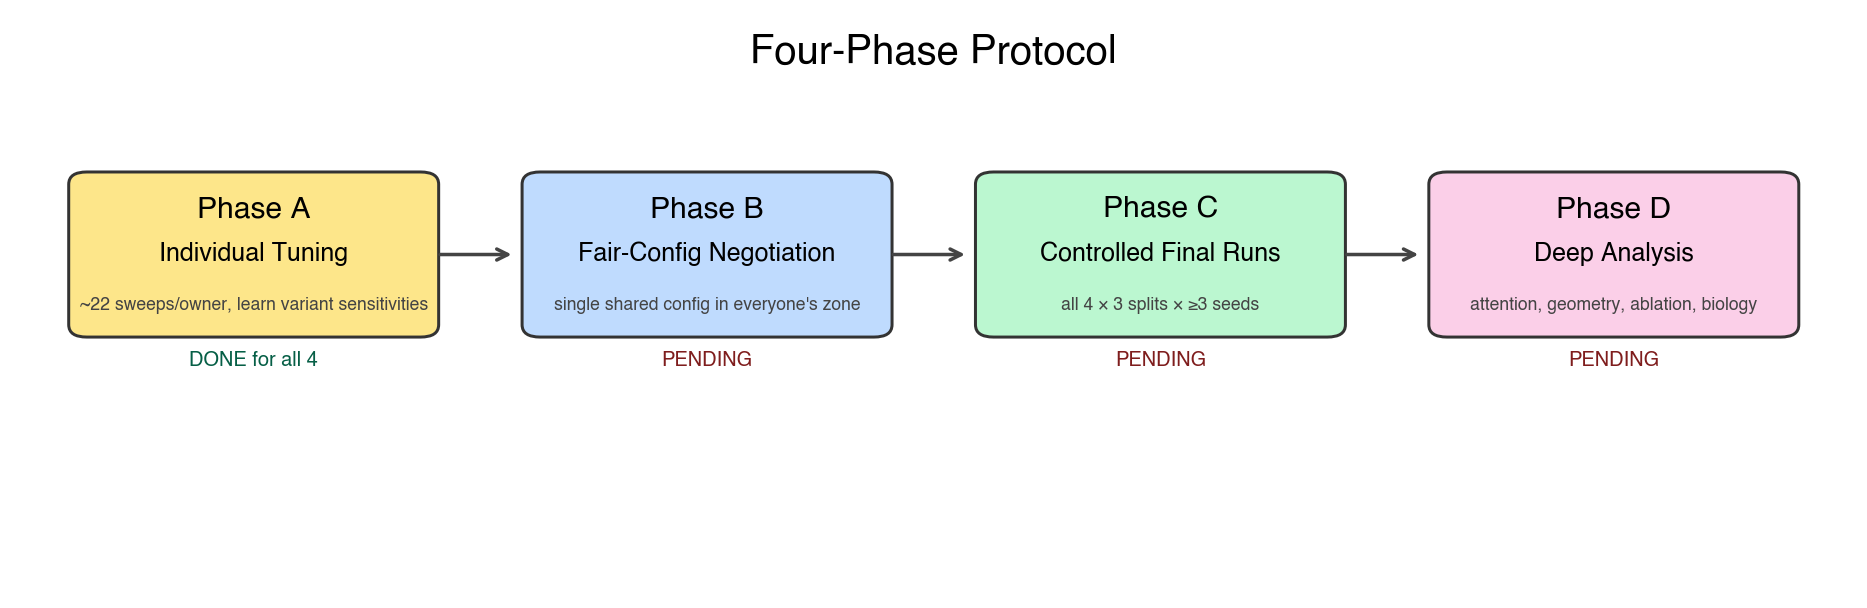
\includegraphics[width=0.99\linewidth]{poster_figures/diagram_09_pipeline.png}\par\smallskip
  \smallbody\raggedright
  \textbf{A} 88 sweeps $\to$ HP sensitivities. \ \textbf{B} Negotiate
  \emph{fair config}. \ \textbf{C} 4\,var $\times$ 3\,splits $\times$
  3\,seeds = \textbf{36 runs} at locked config. \ \textbf{D} Extract
  attention, predictions, hidden states, gradients, CKA.\par\smallskip
  \callout{\smallbody\color{lilacDark}
    \textbf{Locked:} $d{=}128$, $h{=}4$, $L{=}6$\,/\,$3{+}3$,
    lr$\,{=}3{\times}10^{-4}$, dropout $0.1$, bs $64$, 30 ep.,
    AdamW + cosine + 500-step warmup, seeds 42/123/456.\
    \textbf{Compute:} NYU HPC, 2$\times$ A100, $\sim$57 GPU-h
    ($\sim$4.7\,\% of 1{,}200-h budget; $\sim$7\,kg CO$_2$-eq).\
    \textbf{All four phases complete.}}

  % --- f) Convergence Sanity ------------------------------------------
  \subhead{f) Convergence Sanity --- All Variants Train Cleanly}
  \centering
  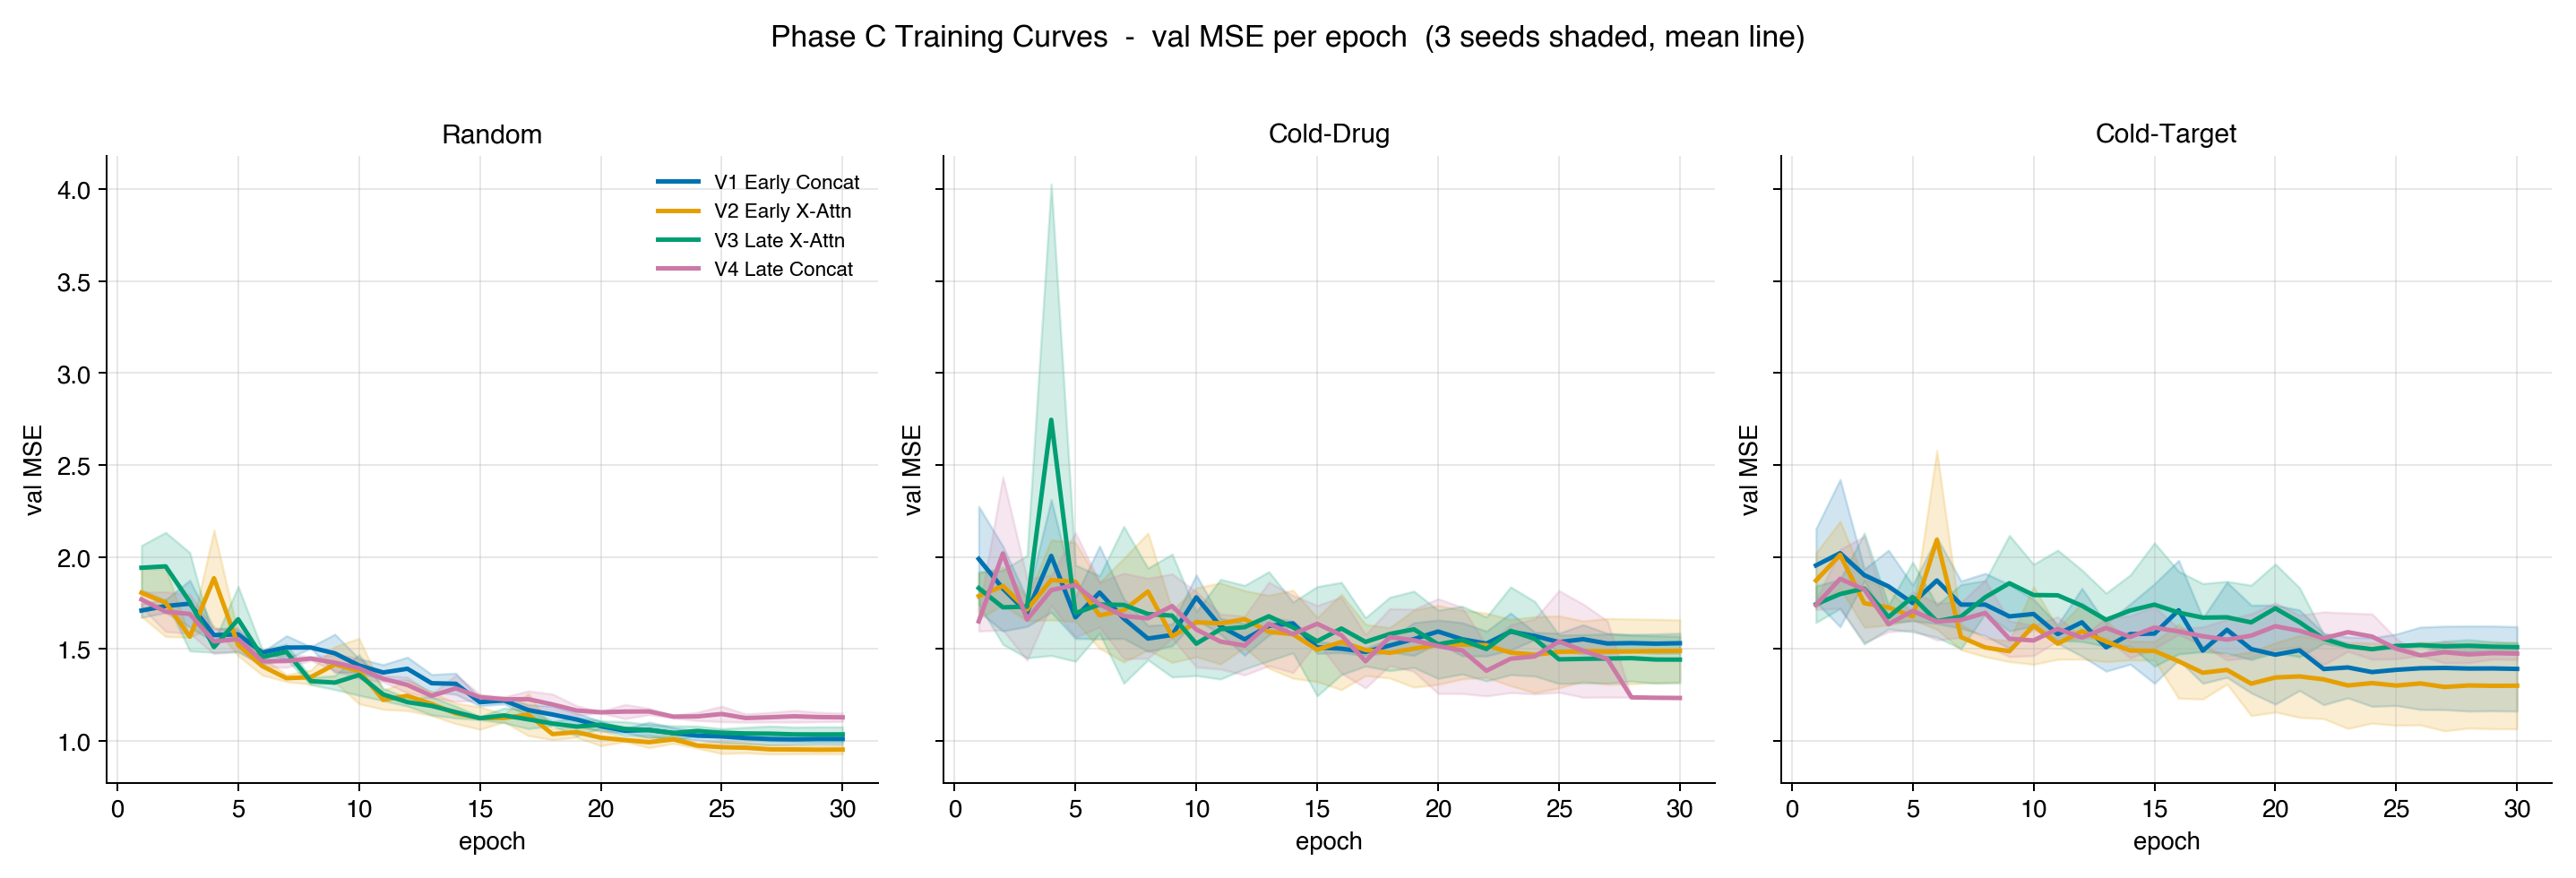
\includegraphics[width=0.85\linewidth]{poster_figures/diagram_12_loss_curves.png}
  \figcap{Train + val MSE per epoch on the random split. All four
  variants drop from $\sim$14 (epoch 1) to $\sim 1.0$--$1.5$
  (epoch 30) without divergence or oscillation. \textbf{No variant is
  harder to optimize} --- the locked Phase B config is inside every
  variant's safe zone, so any cross-variant gap in Section 8
  attributes to architecture, not to optimization difficulty.}
}

% =====================================================================
%  COLUMN 3 --- WHAT (results + deep analysis, findings, conclusions)
% =====================================================================
\column{0.33}

\block{8.\ Results \& Deep Analysis}{%
  \subheadFirst{a) Headline Numbers --- Phase C, 36 Runs}
  \smallbody\centering
  \renewcommand{\arraystretch}{1.25}
  \setlength{\tabcolsep}{2pt}
  \begin{tabular}{@{}p{2.9cm} >{\centering\arraybackslash}p{3.0cm}
                              >{\centering\arraybackslash}p{3.0cm}
                              >{\centering\arraybackslash}p{3.0cm}@{}}
  \toprule
  \textbf{Variant} & \textbf{Random}\,$\downarrow$ &
  \textbf{Cold-Drug}\,$\downarrow$ & \textbf{Cold-Tgt}\,$\downarrow$ \\
  \midrule
  \Vone\ Early Con   & 1.004\,$\pm$\,0.031 & 1.476\,$\pm$\,0.029 & 1.360\,$\pm$\,0.197 \\
  \rowcolor{lilacPale}
  \Vtwo\ Early X-A & \textbf{0.948}\,$\pm$\,\textbf{0.023}\,$\bigstar$ & 1.432\,$\pm$\,0.170 & \textbf{1.248}\,$\pm$\,\textbf{0.187}\,$\bigstar$ \\
  \Vthree\ Late X-A  & 1.030\,$\pm$\,0.039 & \textbf{1.410}\,$\pm$\,\textbf{0.129}\,$\bigstar$ & 1.549\,$\pm$\,0.131 \\
  \Vfour\ Late Con   & 1.119\,$\pm$\,0.018 & 1.465\,$\pm$\,0.178 & 1.467\,$\pm$\,0.069 \\
  \bottomrule
  \end{tabular}
  \figcap{Mean $\pm$ std (3 seeds). $\bigstar$ = best per column.
  \Vtwo\ wins 2 splits; \Vthree\ wins cold-drug;
  \textbf{\Vfour\ (field default) never wins}.}

  \subhead{b) MSE per Split --- All Four Variants}
  \centering
  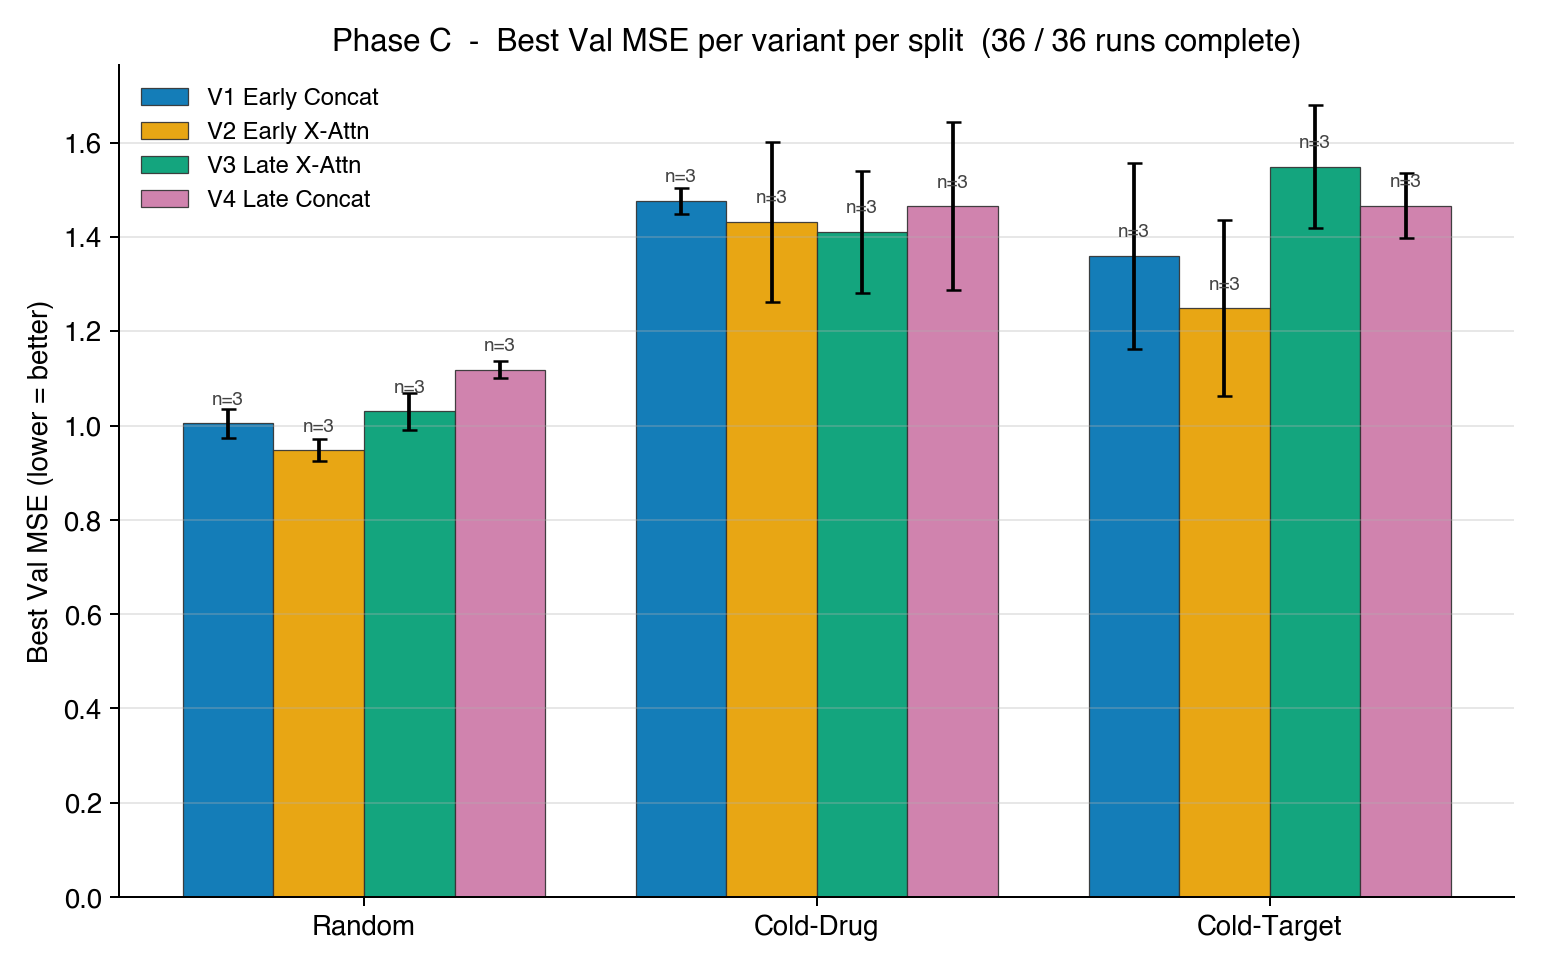
\includegraphics[width=0.8\linewidth]{poster_figures/diagram_10b_mse_per_split.png}
  \figcap{Bars = mean MSE across 3 seeds; whiskers = $\pm$ 1 std.
  Cross-attention (\Vtwo, \Vthree) wins every split. Concatenation
  (\Vone, \Vfour) wins none. Cold splits cost +40\,\% MSE on average.}

  \subhead{\boldmath c) The CKA Finding --- Stage $\succ$ Mechanism \unboldmath}
  \centering
  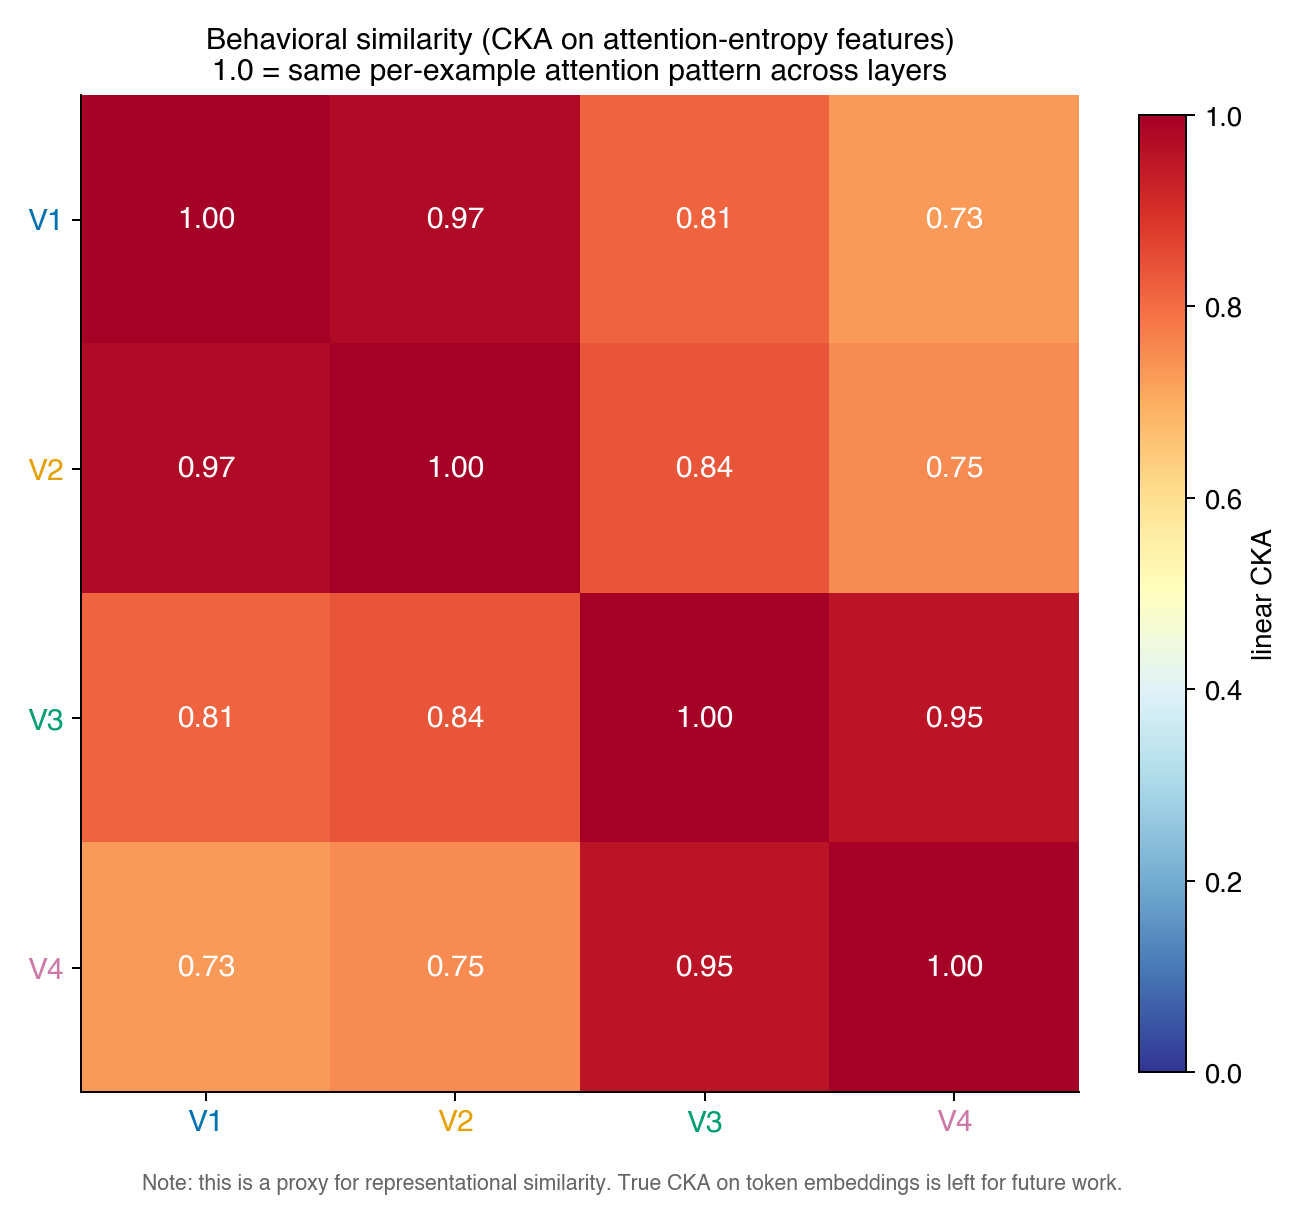
\includegraphics[width=0.40\linewidth]{poster_figures/diagram_18_cka_matrix.png}
  \highlight{\smallbody\color{lilacDark}
    Linear CKA (256 held-out pairs):\;
    $\{$\Vone, \Vtwo$\}$ early \textbf{0.97};\;
    $\{$\Vthree, \Vfour$\}$ late \textbf{0.95};\;
    cross-cluster \textbf{0.73--0.84}.\\[1pt]
    \textbf{Refutes H4.} The $2{\times}2$ collapses to a $1{\times}2$:
    fusion stage drives behavior, not mechanism.}

  \subhead{d) Mechanism --- Attention Entropy \& Mixing-Point}
  \centering
  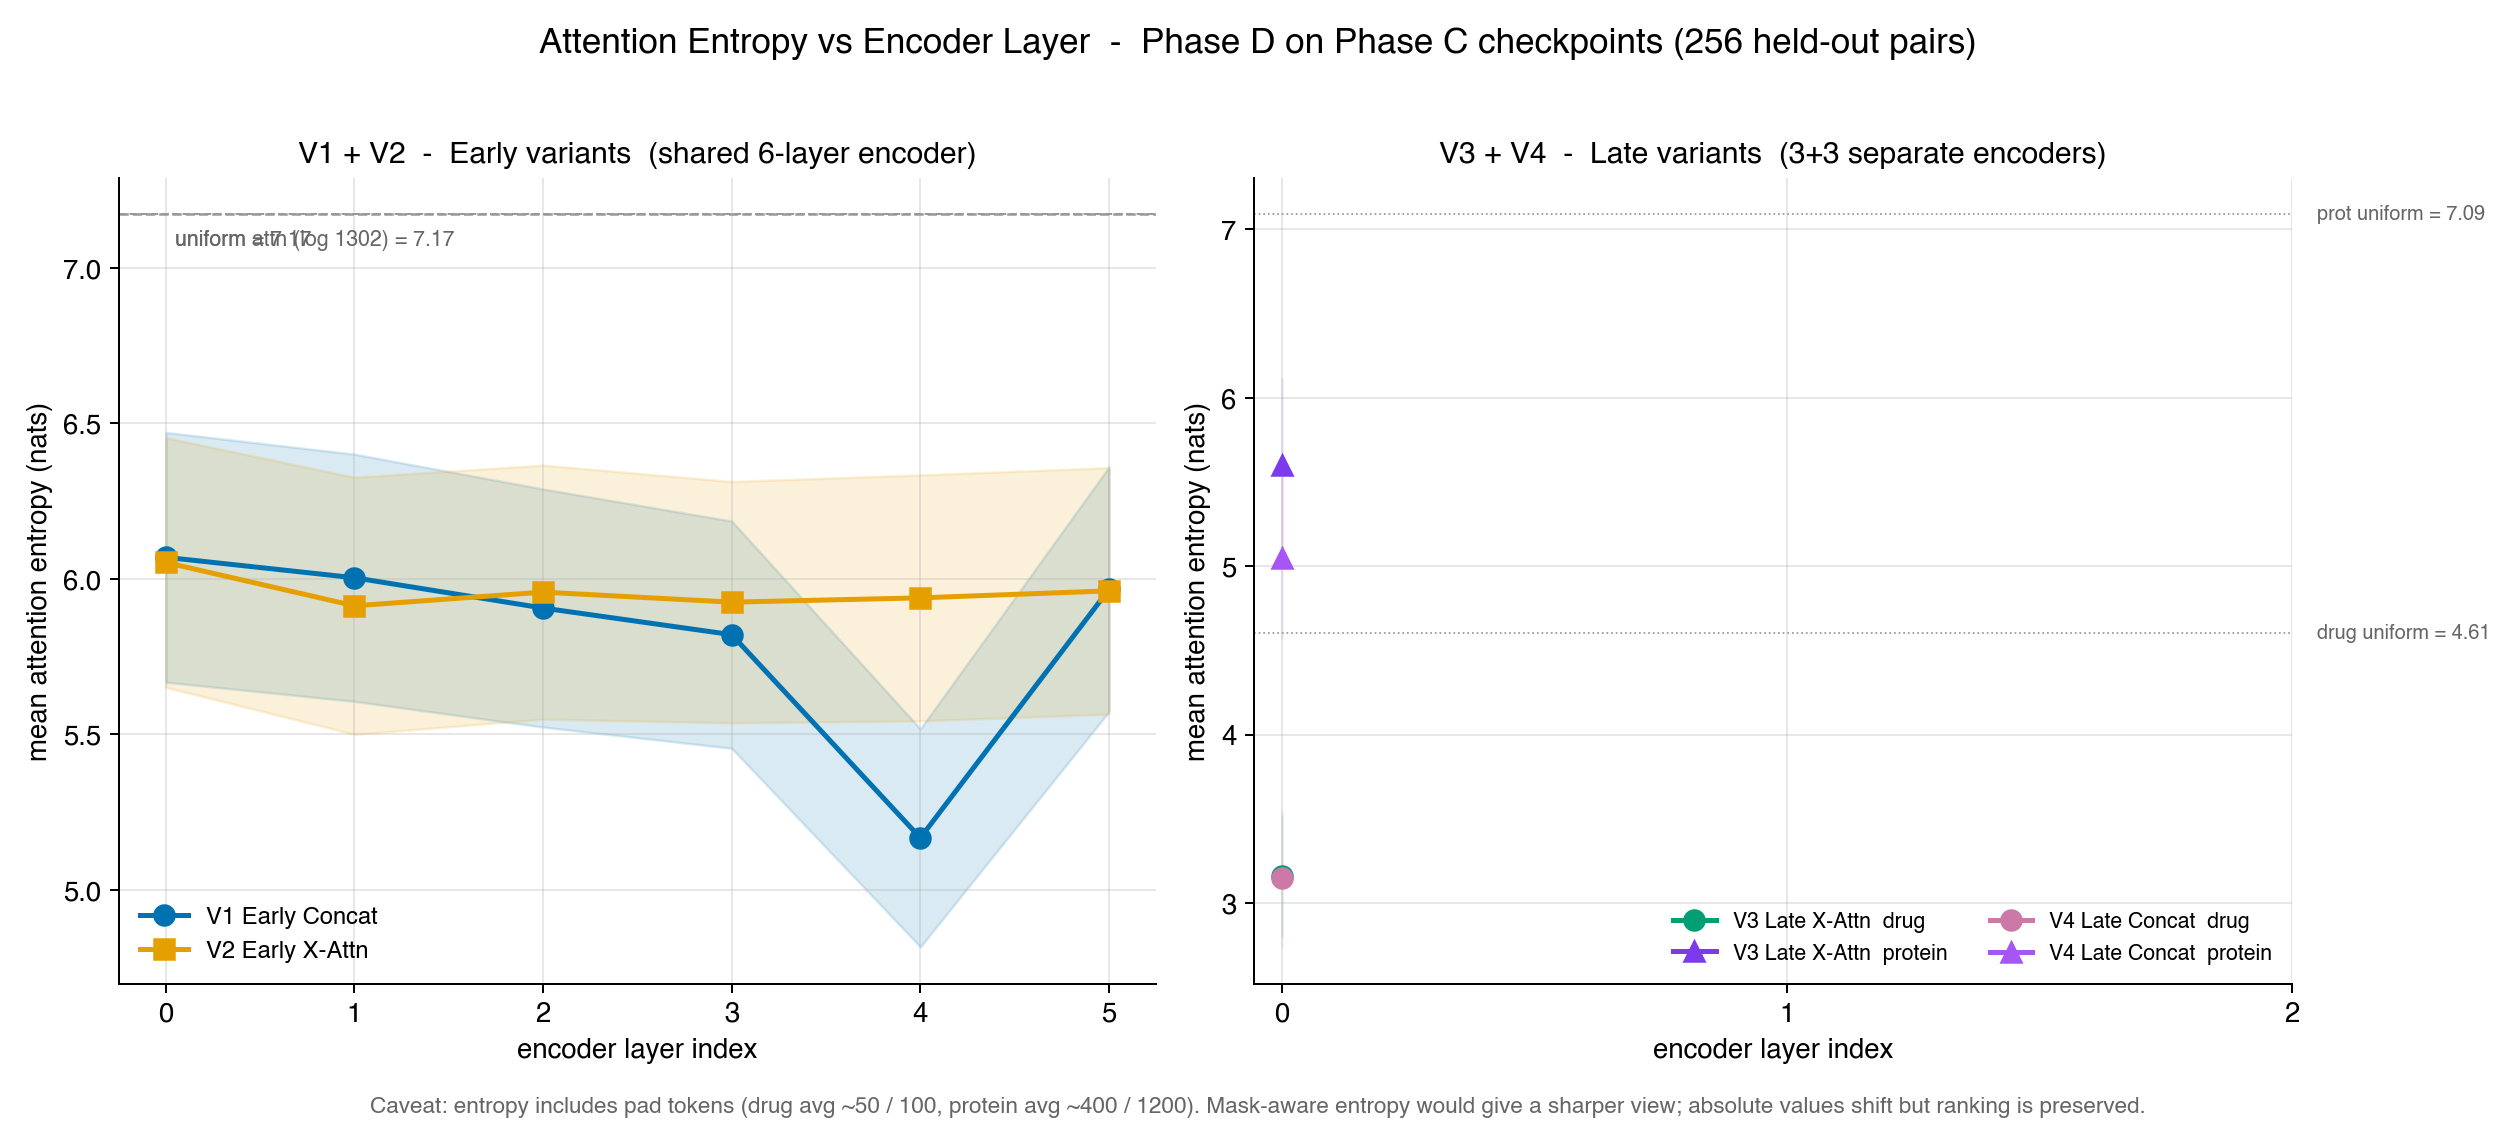
\includegraphics[width=0.495\linewidth]{poster_figures/diagram_16_attention_entropy.png}\hfill
  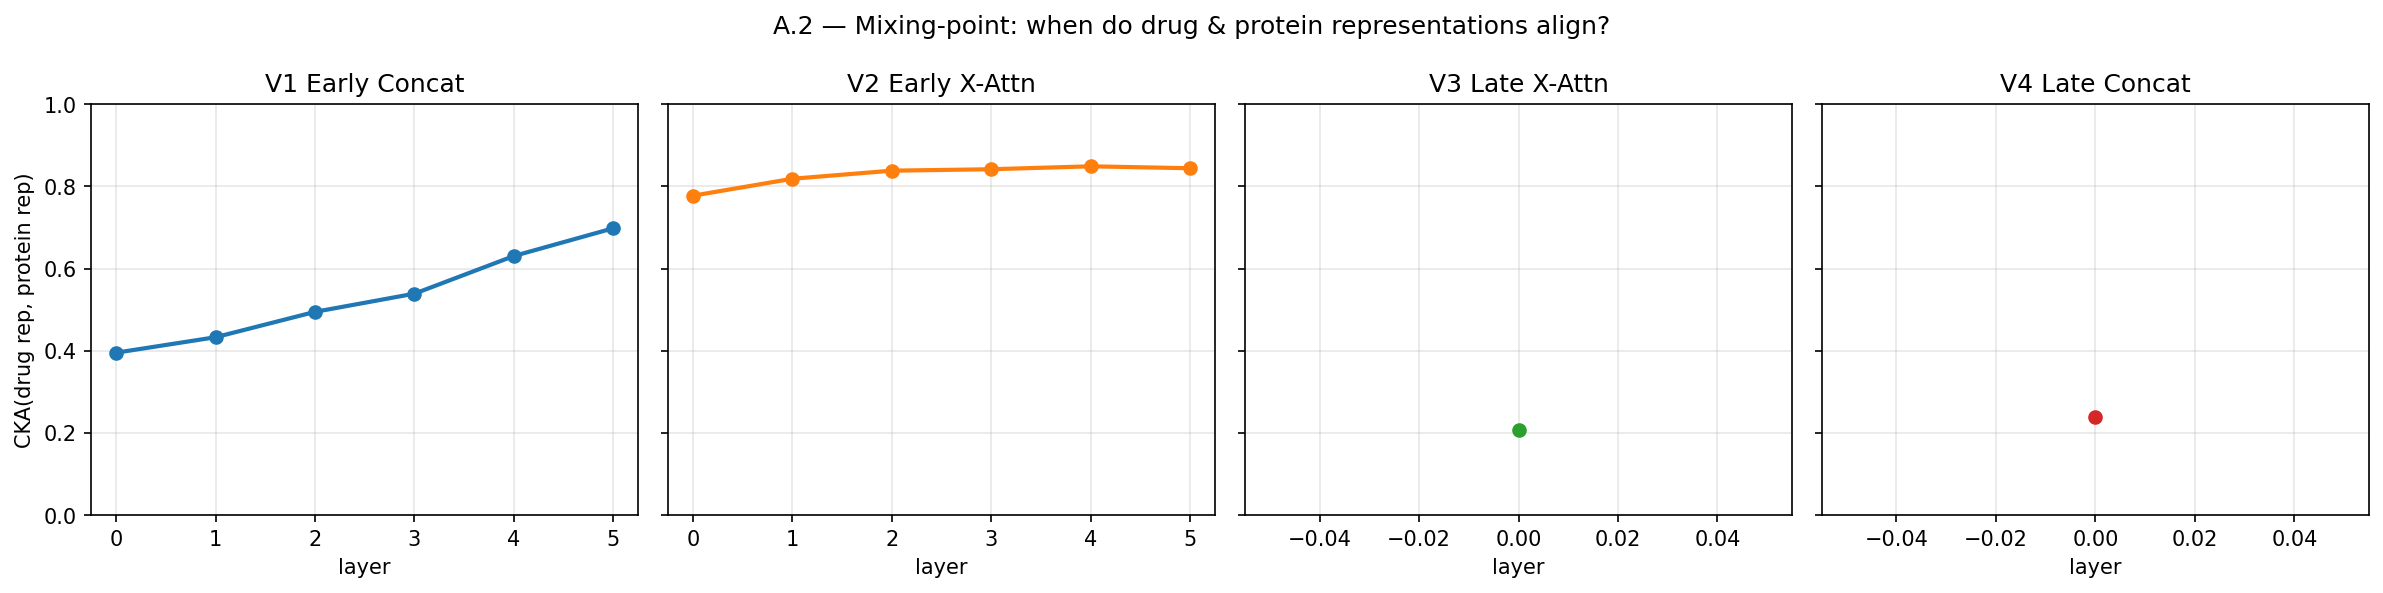
\includegraphics[width=0.495\linewidth]{poster_figures/diagram_19_mixing_point.png}
  \figcap{\textbf{Left:} \Vone's encoder shows depth-specialization
  (entropy dip at L4); \Vtwo\ stays flat $\sim$6.0 nats across all
  six layers. \textbf{Right:} drug$\leftrightarrow$protein CKA per
  layer. \Vtwo\ starts at \textbf{0.78} (cross-attn block hands the
  encoder pre-aligned modalities); \Vone\ climbs from \textbf{0.40
  $\to$ 0.70} across six layers; \Vthree\,/\,\Vfour\ never align
  (CKA $\sim$0.21--0.24). \textbf{Mechanism explained:} early X-attn
  removes the encoder's burden of learning alignment.}

  \subhead{e) Failure Modes --- Where Each Variant Breaks}
  \centering
  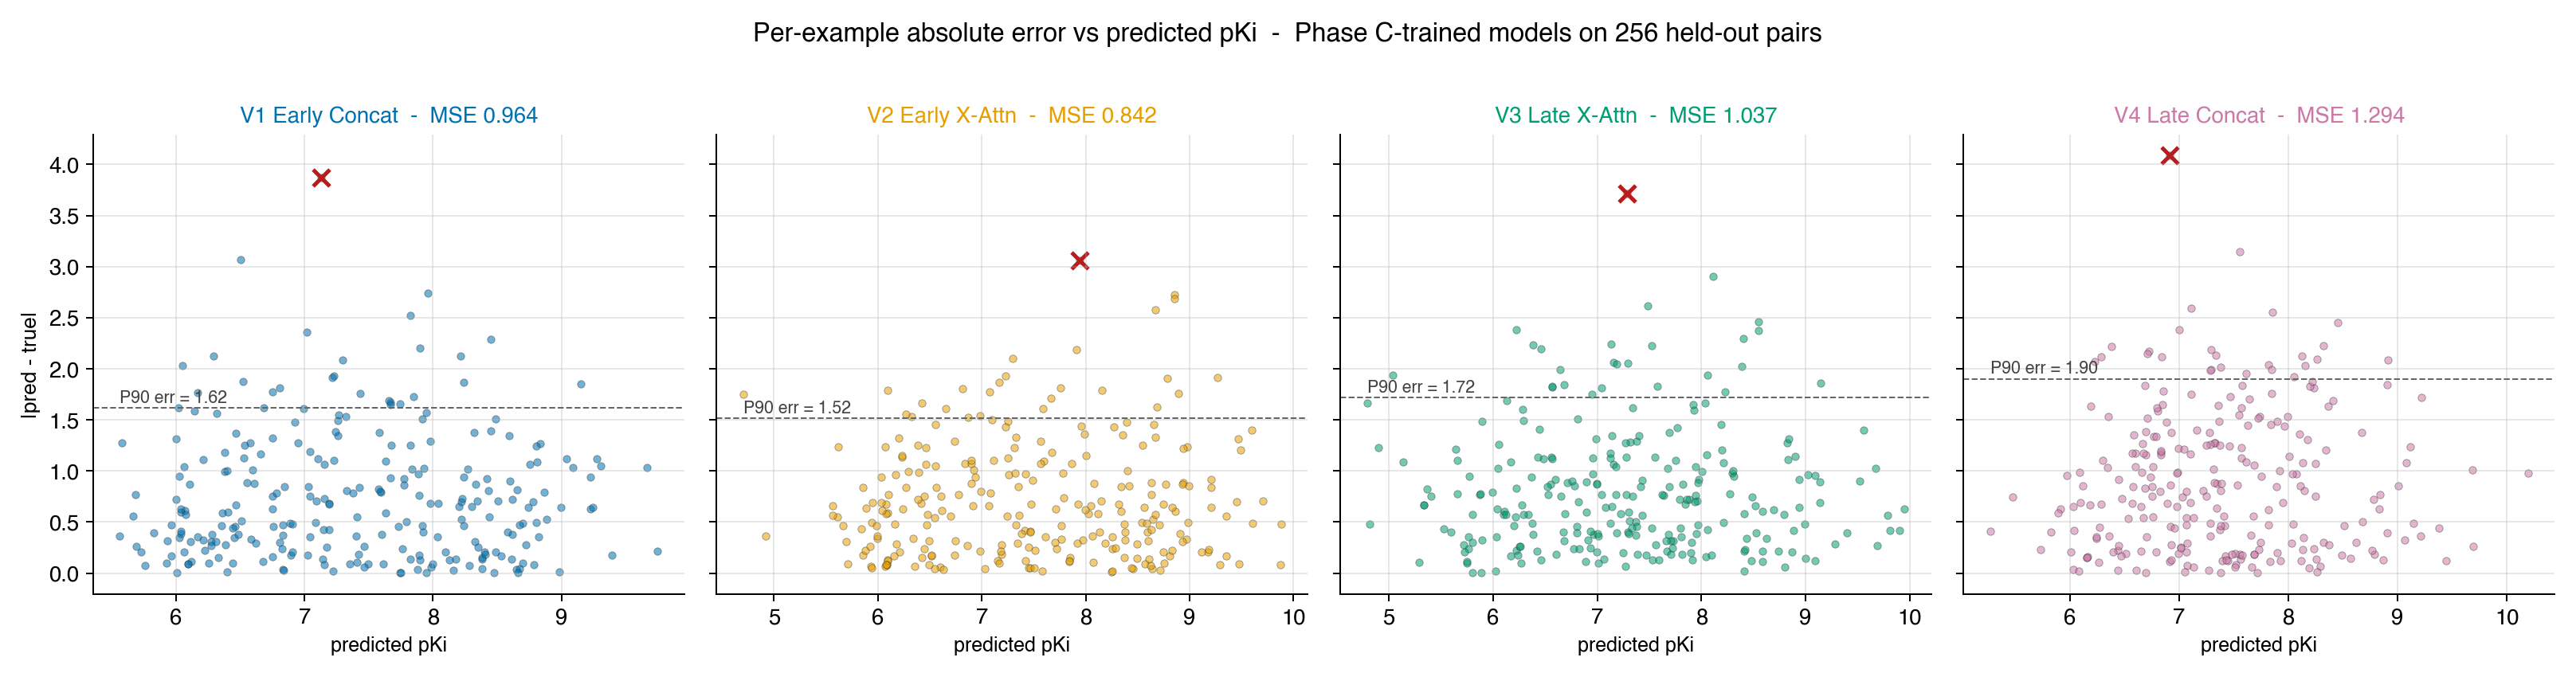
\includegraphics[width=0.495\linewidth]{poster_figures/diagram_27_error_stratification.png}\hfill
  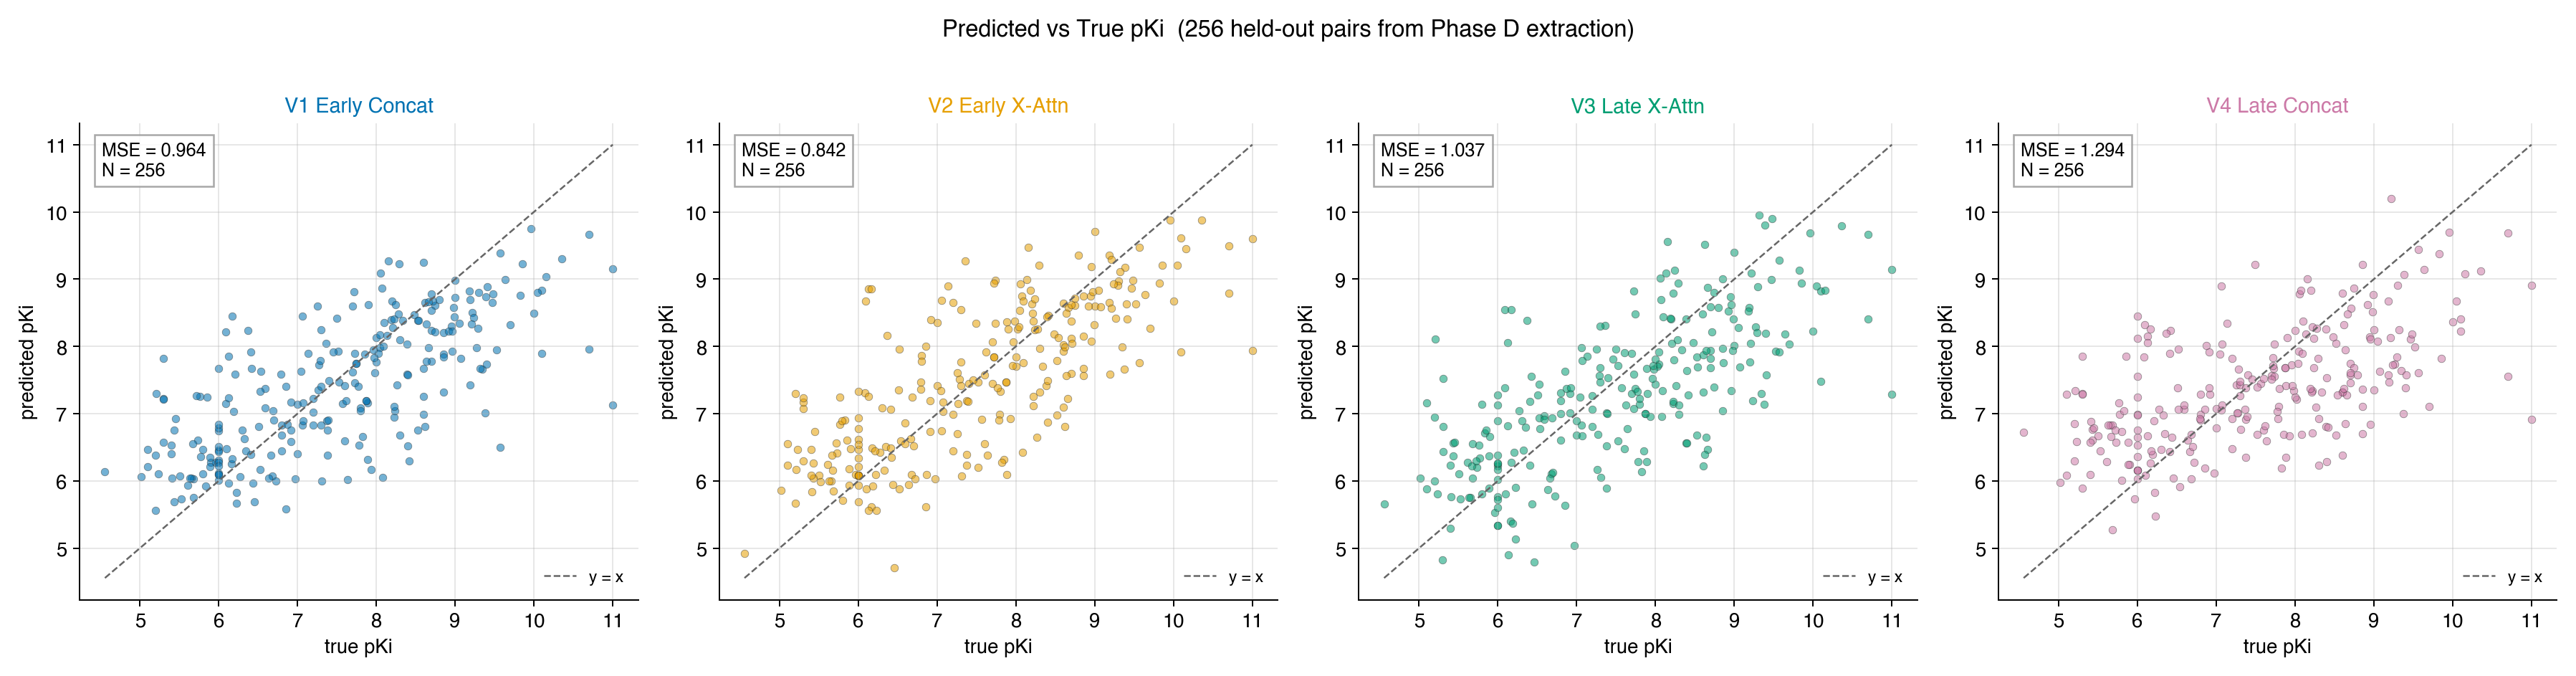
\includegraphics[width=0.495\linewidth]{poster_figures/diagram_13_predicted_vs_true.png}
  \figcap{\textbf{Left:} error stratified by drug + protein length.
  \Vtwo\ has the lowest P90 error (1.52) and lowest worst residual
  (3.05); \Vfour\ fails most catastrophically on long proteins.
  \textbf{Right:} predicted vs true on cold-target (the hardest
  split). Tails reveal per-variant failure regimes ---
  \Vtwo's points hug the diagonal tightest; \Vfour\ shows
  systematic under-prediction at high pKi.}
}

\block{9.\ Findings \& Conclusions}{%
  \bodysize
  \textbf{What we asked.} Does the \emph{stage} (before vs after
  encoding) and \emph{mechanism} (concat vs X-attn) of cross-modal
  fusion change a transformer DTI model's accuracy, generalization,
  and learned representations?\par\smallskip

  \textbf{What we found --- five claims, each measured.}
  \smallbody
  \begin{enumerate}[leftmargin=0.6cm, itemsep=3pt, topsep=2pt]
    \item \textbf{No Pareto-optimal architecture.} Each split has a
      different winner. \Vtwo\ wins random + cold-target, \Vthree\
      wins cold-drug, \Vfour\ (field default) wins zero. Architecture
      choice should depend on \emph{deployment scenario}.
    \item \textbf{Cross-attention $>$ concatenation, on every split.}
      \Vtwo\ + \Vthree\ collectively win 3 of 3; \Vone\ + \Vfour\
      win 0 of 3. The $\sim$10\,\% extra X-attn parameters earn
      their cost.
    \item \textbf{Stage $\succ$ Mechanism (the deep finding).} CKA
      clusters by stage (within-cluster $\geq 0.95$), not by
      mechanism (across-cluster 0.73--0.84). The $2\times 2$ design
      collapses behaviorally to a $1\times 2$.
    \item \textbf{Mechanism explained.} Mixing-point CKA shows
      \Vtwo's pre-encoder cross-attn block delivers
      drug$\leftrightarrow$protein alignment of \textbf{0.78 at
      layer 0}, where \Vone\ takes 6 layers to climb from 0.40 to
      0.70. \Vtwo's flat attention-entropy curve is the
      \emph{symptom}; the upstream alignment is the \emph{cause}.
    \item \textbf{\Vone\ is the parameter-efficient sweet spot;
      \Vfour\ is the most reliable.} \Vone: 1.27\,M params, single
      shared encoder, beats \Vfour\ on every split. \Vfour: lowest
      seed variance ($\sigma\leq 0.07$ on 2 of 3 splits) but
      highest mean MSE --- usable when ranking-stability matters.
  \end{enumerate}\par\smallskip

  \bodysize
  \textbf{Why it matters.} Switching from the field-default \Vfour\
  to early-fusion cross-attention (\Vtwo) yields a \textbf{15\,\%
  relative MSE reduction on random} and \textbf{17\,\% on
  cold-target} --- the most realistic deployment scenario. The
  six-axis mechanistic dissection (information flow, geometry,
  attention, gradients, mixing-point, error modes) explains
  \emph{why}, not just \emph{what}.
}

\block{10.\ Future Work}{%
  \smallbody
  \textbf{Limitations.} Single-dataset training (BindingDB Ki,
  21\,\% censored at pKi $= 5.0$); sequence-only inputs (no 3D
  structure, no pre-trained encoders); modest scale ($d{=}128$,
  1.2--1.4\,M params); causal head/layer ablations and binding-site
  recovery vs PDBbind out of scope; pad tokens included in attention
  entropy.\par\smallskip

  \textbf{Future Work.}
  \begin{itemize}[leftmargin=0.6cm, itemsep=1pt, topsep=2pt]
    \item Multi-modal drug input: SMILES + molecular graph (GNN) +
          3D conformer.
    \item Pre-trained encoders (ChemBERTa + ESM-2) --- does
          pre-training neutralize the fusion-stage gap?
    \item Causal interventions on Phase C ckpts: head / layer
          ablation, representation swap ($\sim$3 GPU-h per variant).
    \item Binding-site recovery vs PDBbind: Precision@K on
          attention-as-attribution.
    \item Agentic drug optimization: best DTI model wrapped as a
          tool inside an LLM lead-optimization agent.
  \end{itemize}
}

\block{11.\ Acknowledgements}{%
  \smallbody
  \textbf{Acknowledgements.} NYU HPC for cloud-burst GPU access
  ($\sim$57 GPU-h). Course staff of CSCI-2565 \emph{Machine
  Learning}: Prof.\ Rajesh Ranganath (instructor); Nhi Nguyen,
  Riya Mahesh, Siddhant Mohan (TAs). BindingDB and the Psychoactive
  Drug Screening Program (PDSP) for the public dataset.\par\smallskip

  \fontsize{11}{14}\selectfont
  \textbf{References.}
  [1] Vaswani \emph{et al.} \emph{Attention is All You Need},
  NeurIPS 2017.\
  [2] Kornblith \emph{et al.} \emph{CKA}, ICML 2019.\
  [3] Huang \emph{et al.} \emph{MolTrans}, Bioinformatics 2021.\
  [4] Huang \emph{et al.} \emph{DeepPurpose}, Bioinformatics 2020.\
  [5] Bai \emph{et al.} \emph{DrugBAN}, Nat.\ Mach.\ Intell.\ 2023.\
  [6] Zhao \emph{et al.} \emph{HyperAttentionDTI}, Bioinformatics 2022.\
  [7] Nguyen \emph{et al.} \emph{PerceiverCPI}, 2022.\
  [8] Chen \emph{et al.} \emph{TransformerCPI}, Bioinformatics 2020.\
  [9] Liu \emph{et al.} \emph{BindingDB 2023}, NAR 2023.\
  [10] Davis \emph{et al.}, Nat.\ Biotech.\ 2011.\
  [11] Pahikkala \emph{et al.}, Brief.\ Bioinform.\ 2015.\
  [12] Mayr \emph{et al.}, Chem.\ Sci.\ 2018.\
  [13] Lin \emph{et al.} \emph{ESM-2}, Science 2023.\
  [14] Chithrananda \emph{et al.} \emph{ChemBERTa}, 2020.\
  [15] Sundararajan \emph{et al.} \emph{Integrated Gradients}, ICML 2017.
  \par\smallskip
  \centering
  {\fontsize{12}{15}\selectfont\rmfamily\color{warmgray}
   Contact: bhaveshgupta01@gmail.com \,\textbullet\, NYU Courant
   \,\textbullet\, Spring 2026
   \,\textbullet\, full repo + 27 figures via QR in Column 1}
}

\end{columns}

\end{document}
